%-------------------------------------------------------------------------------
%                      Template Naskah Skripsi
%               	Berdasarkan format JTETI FT UGM
% 						(c) @gunturdputra 2014
%-------------------------------------------------------------------------------

%Template pembuatan naskah skripsi.
\documentclass{jtetiskripsi}

%Untuk prefiks pada daftar gambar dan tabel
\usepackage[titles]{tocloft}
\renewcommand\cftfigpresnum{Gambar\  }
\renewcommand\cfttabpresnum{Tabel\   }

%Untuk hyperlink dan table of content
\usepackage{hyperref}
\newlength{\mylenf}
\settowidth{\mylenf}{\cftfigpresnum}
\setlength{\cftfignumwidth}{\dimexpr\mylenf+2em}
\setlength{\cfttabnumwidth}{\dimexpr\mylenf+2em}

%Untuk Bold Face pada Keterangan Gambar
\usepackage[labelfont=bf]{caption}

%Untuk caption dan subcaption
\usepackage{caption}
\usepackage{subcaption}

%pdf
\usepackage{pdfpages}

%table
\usepackage{graphics}

\usepackage{wrapfig}

%-----------------------------------------------------------------
%Disini awal masukan untuk data proposal skripsi
%-----------------------------------------------------------------
\titleind{PERANCANGAN APLIKASI SISTEM INFORMASI MANAJEMEN PROGRAM KERJA OPMAWA FMIPA UNIVERSITAS NEGERI JAKARTA}

\fullname{Maulana Rahman Nur}

\idnum{3145151011}

\approvaldate{26 Juni 2018}

\degree{Sarjana Ilmu Komputer}

\yearsubmit{2018}

\program{Ilmu Komputer}

\dept{Ilmu Komputer}

\firstsupervisor{Drs. Mulyono, M.Kom.}
\firstnip{196605171994031003}

\secondsupervisor{Ratna Widyati, S.Si, M.Kom.}
\secondnip{197509252002122002}

%hypenation

\hyphenation{Al-go-rit-ma pe-san kom-pre-si di-gu-na-kan seg-men di-rep-re-sen-ta-si-kan di-kem-bang-kan di-sem-bu-nyi-kan eks-trak-si meng-gu-na-kan bi-lang-an pe-ri-o-de di-ma-suk-kan a-kan me-nga-la-mi pe-rang-kat di-pub-li-ka-si-kan di-la-ku-kan mem-be-ri-kan di-si-sip-kan }

%-----------------------------------------------------------------
%Disini akhir masukan untuk data proposal skripsi
%-----------------------------------------------------------------

\begin{document}

\cover

\chapter*{\centering{\large{LEMBAR PENGESAHAN}}}
\thispagestyle{empty} {\bf }Dengan ini saya mahasiswa Fakultas
Matematika dan Ilmu Pengetahuan Alam, Universitas Negeri Jakarta

\vskip3mm

\begin{tabular}{lll}
  Nama 			& : & Maulana Rahman Nur \\
  No. Registrasi& : & 3145151011 \\
  Jurusan 		& : & Ilmu Komputer \\
  Judul 		& : & Perancangan Aplikasi Sistem Informasi Manajemen Program \\
  & &  Kerja Opmawa FMIPA Universitas Negeri Jakarta.
\end{tabular}

\vskip3mm

\noindent Menyatakan bahwa proposal ini telah siap diajukan untuk sidang proposal.
%\begin{center}
%Menyatakan bahwa skripsi ini telah siap diajukan untuk sidang skripsi.
%\end{center}



\begin{center}
\vskip3mm

Menyetujui,

\vskip3mm
\begin{spacing}{1.25}

\begin{tabular}{ccc}
  \hskip-2mm Dosen Pembimbing I & \qquad \qquad \qquad \qquad \qquad & \hskip-6mm Dosen Pembimbing II \\
   &  &  \\
   &  &  \\
   &  &  \\
   &  &  \\
  \hskip-2mm \underline{\textbf{Drs. Mulyono, M.Kom.}} &  & \hskip-6mm \underline{\textbf{Ratna Widyati, S.Si, M.Kom.}} \\
  \hskip-2mm NIP. 19660517 199403 1 003 &  & \hskip-6mm NIP. 19750925 200212 2 002	 \\
\end{tabular}
\end{spacing}
\end{center}
\vskip3mm
\begin{center}
Mengetahui, \\
Ketua Program Studi Ilmu Komputer
\end{center}
\begin{spacing}{1.25}
{ \ }
\\
\\
{ \ }\begin{center}
\underline{\textbf{Ir. Fariani I., M.T.}} \\
{NIP. 19600211 198703 2 001}
\end{center}
\end{spacing} 
%\chapter*{\centering{\large{\thesisapprovalname}}}
\thispagestyle{empty} {\bf }
\vspace{-0.5cm}
\begin{center}
	\textbf{Implementasi Steganografi pada Citra \emph{Digital} \\ dengan Metode \emph{Least Significant Bit}}
\end{center}

\vspace{1mm}
\vskip 1.5mm \noindent
\begin{tabular}{ll}
	\hskip-2mm Nama & : Amelia Apriliani \\
	\hskip-2mm No. Registrasi & : 3145143626 \\
\end{tabular}


\vskip2mm

\noindent \begin{flushleft}
	\begin{tabular}{llcc}
		
		& \hskip15mm Nama & Tanda Tangan & Tanggal \\
		
		\hskip-1cm Penanggung Jawab &  &  &  \\
		\hskip-1cm Dekan & : Prof. Dr. Suyono, M.Si. & ............... & ............. \\
		& \hskip3mm NIP. 19671218 199303 1 005 &  &  \\
		\hskip-1cm Wakil Penanggung Jawab &  &  &  \\
		\hskip-1cm Wakil Dekan I & : Dr. Muktiningsih, M.Si. & ............... & ............. \\
		& \hskip3mm NIP. 19640511 198903 2 001 &  &  \\
		\hskip-1cm Ketua & : Ir. Fariani Hermin I, M.T. & ............... & ............. \\
		& \hskip3mm NIP. 19600211 198703 2 001 &  &  \\	
		\hskip-1cm Sekretaris & : Med Irzal, M.Kom. & ............... & ............. \\
		& \hskip3mm NIP. 19770615 200312 1 001 &   &  \\
		\hskip-1cm Penguji & : Ria Arafiah, M.Si. & ............... & ............. \\
		& \hskip3mm NIP. 19751121 200501 2 004 &  &  \\
		\hskip-1cm Pembimbing I & : Drs. Mulyono, M.Kom. & ............... & ............. \\
		& \hskip3mm NIP. 19660517 199403 1 003 &  &  \\
		\hskip-1cm Pembimbing II & : Ratna Widyati, S.Si, M.Kom. & ............... & ............. \\
		& \hskip3mm NIP. 19750925 200212 2 002 &  &  \\
	\end{tabular}
\end{flushleft}

\vskip1mm

\noindent Dinyatakan lulus ujian skripsi tanggal: 09 Agustus 2018


\chapter*{\centering{\large{LEMBAR PERNYATAAN}}}

Saya menyatakan dengan sesungguhnya bahwa skripsi dengan judul \textbf{"Perancangan Aplikasi Sistem Informasi Manajemen Program Kerja OPMAWA FMIPA Universitas Negeri Jakarta"} yang disusun sebagai syarat untuk memperoleh gelar Sarjana komputer dari Program Studi Ilmu Komputer Universitas Negeri Jakarta adalah karya ilmiah saya dengan arahan dari dosen pembimbing.

Sumber informasi yang diperoleh dari penulis lain yang
telah dipublikasikan yang disebutkan dalam teks skripsi ini, telah dicantumkan dalam Daftar Pustaka sesuai dengan norma, kaidah dan etika penulisan ilmiah.

Jika dikemudian hari ditemukan sebagian besar skripsi ini bukan hasil karya saya sendiri dalam bagian-bagian tertentu, saya bersedia menerima sanksi pencabutan gelar akademik yang saya sanding dan sanksi-sanksi lainnya sesuai dengan peraturan perundang-undangan yang berlaku.

\vspace{.5cm}

\begin{tabular}{p{7.5cm}c}
	&Jakarta, 13 September 2019\\
	&\\
	&\\
	&\\
	&Maulana Rahman Nur
\end{tabular}

%-----------------------------------------------------------------
%Disini awal masukan Acknowledment
%-----------------------------------------------------------------
%\acknowledgment
%TEST
%\begin{flushright}
%	\emph{Untuk Ayah, Mama,\\dan Adikku tercinta.}
%\end{flushright}
%-----------------------------------------------------------------
%Disini awal masukan untuk Prakata
%-----------------------------------------------------------------

%\preface

%Puji syukur penulis panjatkan ke hadirat Allah SWT Tuhan Yang Maha Kuasa karena hanya dengan ridha-Nya, Skripsi ini dapat terselesaikan tanpa halangan berarti. Keberhasilan dalam menyusun Skripsi ini tidak lepas dari bantuan berbagai pihak yang mana dengan tulus dan ikhlas memberikan masukan yag bermanfaat dalam proses penyusunan Skripsi ini. Jenis penelitian yang dipilih adalah kajian teori dengan judul Perancangan Aplikasi Sistem Informasi Manajemen Program Kerja OPMAWA FMIPA Universitas Negeri Jakarta.

%Terima kasih penulis ucapkan kepada Bapak Drs. Mulyono, M.Kom dan Ibu Ratna Widyati, S.Si, M.Kom selaku pembimbing I dan pembimbing II yang telah memberikan banyak bantuan, bimbingan, serta arahan dalam penyelesaian tugas akhir ini. Terima kasih pula kepada Pembimbing Akademik Ibu Ria Arafiah, M.Si yang telah membimbing penulis secara akademik selama kuliah di Program Studi Ilmu Komputer UNJ. Di samping itu penghargaan penulis disampaikan ke seluruh Dosen Prodi Ilmu Komputer FMIPA UNJ yang tidak bisa disebutkan satu per satu, atas ilmu dan bimbingannya selama penulis berkuliah di Ilmu Komputer UNJ. 

%Ungkapan terima kasih disampaikan kepada Ayah dan ibu yang selama ini selalu mendoakan dan memberikan dukungan kepada penulis tanpa kenal lelah untuk selama-lamanya. Penulis juga mengucapkan terimakasih kepada Evita Dwi oktaviani

%Penulis menyadari bahwa penyusunan Skripsi ini jauh dari sempurna. Akhir kata, teriring permintaan maaf apabila terdapat kesalahan maupun kekeliruan dalam penulisan Skripsi ini. Besar harapan penulis agar Skripsi ini dapat bermanfaat sebagaimana mestinya. Terima kasih.

%\vspace{.5cm}

%\begin{tabular}{p{7.5cm}c}
%	&Jakarta, Agustus 2019\\
%	&\\
%	&\\
%	&\textbf{Penulis}
%\end{tabular}

%-----------------------------------------------------------------
%Disini awal masukan Intisari
%-----------------------------------------------------------------
\begin{abstractind}
\textbf{MAULANA RAHMAN NUR}. Perancangan Aplikasi Sistem Informasi Manajemen Program Kerja Opmawa FMIPA Universitas Negeri Jakarta . Skripsi. Fakultas Matematika dan Ilmu Pengetahuan Alam, Universitas Negeri Jakarta. 2018. Di bawah bimbingan Drs. Mulyono, M.Kom dan Ratna Widyati, S.Si, M.Kom.
\vskip1cm

	Sistem Informasi Manajemen (SIM) merupakan sebuah sistem yang dapat memberikan informasi dalam bentuk laporan dan tampilan kepada pelaku bisnis. Sistem tersebut berfungsi sebagai media yang dapat digunakan sebagai penyambung komunikasi antar pelaku bisnis. Universitas Negeri Jakarta memiliki sebuah Organisasi Mahasiswa (Ormawa) yang disebut sebagai laboratorium kecil pemerintahan dalam kampus yang dinamakan Organisasi Pemerintahan Mahasiswa (Opmawa). Opmawa merupakan sebuah organisasi yang memiliki sistem yang merupakan gambaran dari sistem pemerintahan yang ada di Indonesia. Pada penelitian ini dilakukan analisis kebutuhan berdasarkan permasalahan-permasalahan manajerial di dalam opmawa yang nantinya akan dikembangkan menjadi sebuah sistem yang dapat membantu dalam pendataan dan pengolahan data internal organisasi tersebut  .Sistem berbasis \textit{website} ini dikembangkan dengan menggunakan \textit{framework} Codeigniter yang menganut sistem \textit{Model View Controller} (MVC). Dengan sistem yang sistematis akan membantu setiap anggota dalam sebuah organisasi untuk bekerja sesuai dengan aturan-aturan yang telah ditentukan. 
	
	% Steganografi dapat digunakan sebagai salah satu teknik dalam pengamanan informasi. Steganografi dapat menyembunyikan \emph{file} pesan agar orang awam tidak menyadari keberadaan dari \emph{file} pesan yang disembunyikan. Salah satu metode pada steganografi adalah \emph{Least Significant Bit} (LSB). LSB melakukan penyisipan bit pesan ke dalam bit-bit \emph{file} media yang digunakan. Pada tugas akhir ini, media yang digunakan adalah \emph{file} citra \emph{digital} RGB (\emph{Red, Green} dan \emph{Blue}), dan program dikembangkan dengan menggunakan MATLAB R2016b. Steganografi diawali dengan memasukkan citra \emph{digital} yang akan digunakan, kemudian memasukkan pesan atau \emph{hiddentext} lalu proses penyisipan atau \emph{encoding} dimulai. Setelah proses \emph{encoding} berhasil, citra \emph{digital} disimpan sebagai \emph{stego image}. Untuk mendapatkan kembali pesan maka dilakukan proses \emph{decoding}. Jika proses \emph{decoding} berhasil dilakukan, maka pesan akan ditampilkan. Pada citra \emph{digital} 24 bit dan 32 bit proses penyisipan pesan berhasil dilakukan, sedangkan pada citra \emph{digital} 8 bit proses penyisipan pesan gagal dilakukan. \emph{File} citra hasil steganografi tidak mengalami perubahan yang cukup berarti dari file citra sebelumnya. Sehingga tidak akan menimbulkan kecurigaan dan keamanan pesan tetap terjaga.
	
	\bigskip
	\noindent
	\textbf{Kata kunci :} SIM, manajemen, \textit{website}, \textit{Spiral Model}, \textit{MVC}.
\end{abstractind}

\begin{abstracteng}
\textbf{MAULANA RAHMAN NUR}. Implementation of Steganography in Digital Image with Least Significant Bit Method. Thesis. Faculty of Mathematics and Science, State University of Jakarta. Under supervised by Drs. Mulyono, M.Kom dan Ratna Widyati, S.Si, M.Kom.
\vskip1cm

	\textit{Steganography can be used as one of the techniques in information security. Steganography can combine message files so others do not know of hidden message files. One method of steganography is Least Significant Bit (LSB). LSB inserts message bits into original media files of bits. In this final project, the media is digital image RGB (Red, Green and Blue), and program was developed by using MATLAB R2016b. Steganography begins with entering a digital image that will be used, then entering a message or hiddentext then the insertion or encoding process begins. After the encoding process is successful, the digital image is stored as a stego image. To get the message back the decoding process is carried out. If the decoding process is successful, the message will be displayed. In 24 bit and 32 bit digital image, the encoding process is success, but in 8 bit digital image the process is failed. Stego Image has not significant changes from Cover Image. So it will not cause suspicion and the security of the message is safe.}    
	
	\bigskip
	\noindent
	\textbf{\emph{Keywords :}} \emph{Steganography, message, LSB, digital image}.
\end{abstracteng}
%-----------------------------------------------------------------
%Disini akhir masukan Intisari
%-----------------------------------------------------------------
%-----------------------------------------------------------------

%-----------------------------------------------------------------
%Disini akhir masukan untuk muka skripsi
%-----------------------------------------------------------------

\tableofcontents 
\listoffigures
%\addcontentsline{toc}{chapter}{DAFTAR ISI}
\addcontentsline{toc}{chapter}{DAFTAR GAMBAR}
\listoftables
\addcontentsline{toc}{chapter}{DAFTAR TABEL}

\begin{counterpage}
\end{counterpage}
%Disini awal masukan untuk Bab
%-----------------------------------------------------------------
%!TEX root = ./template-skripsi.tex
%-------------------------------------------------------------------------------
% 								BAB I
% 							LATAR BELAKANG
%-------------------------------------------------------------------------------

\chapter{LATAR BELAKANG}

\section{Latar Belakang}
Manajemen merupakan seluruh upaya dalam mendayagunakan sumber daya untuk mencapai tujuan secara efektif dan efisien \cite{rifai}. Manajemen juga dapat dikatakan sebagai seni atau ilmu dalam mengatur yang memanfaatkan kemampuan orang lain untuk menyelesaikan suatu pekerjaan dengan fungsi-fungsi dari manajemen terhadap usaha yang dilakukan oleh orang lain. Fungsi-fungsi tersebut secara umum dapat berupa tindakan perencanaan, pengorganisasian, Pengarahan dan Pengawasan \cite{rachman}.

Organisasi merupakan sistem yang terpadu yang didalamnya terdapat subsistem dan komponen-komponen yang saling berhubungan. Setiap hubungan yang terjadi merupakan kerjasama diantara subsistem yang ada, sehingga ada saling ketergantungan yang kuat secara internal dan hubungan yang terpadu secara eksternal. Hubungan eksternal itu merupakan bagian dari kenyataan organisasi yang berkaitan dengan lingkungan masyarakat dan elemen lainnya yang mendukung tercapainya tujuan organisasi \cite{priansa}. Definisi tersebut menekankan bahwa organisasi dibuat untuk mewujudkan kebutuhan dan kepentingan masyarakat.

Didalam sebuah organisasi pada umumnya terdiri dari berbagai struktur kepengurusan yang memiliki fungsi dan peranan masing-masing. Seluruh anggota organisasi memerlukan kemampuan dalam memanajemen perannya masing-masing. Fungsi pengorganisasian dalam manajemen tersebut harus memperhatikan kemampuan dari setiap anggota untuk membagi peran dan tugas agar tujuan dari sebuah organisasi dapat tercapai secara efektif. Tanpa adanya manajemen yang baik, pengelolaan dan pengorganisasian tidak akan berjalan secara optimal, sehingga manajemen sangat dibutuhkan di dalam organisasi agar segala tujuan dapat tercapai dengan baik.

Universitas Negeri Jakarta memiliki dua macam organisasi, yakni bersifat organisasi pemerintahan atau yang biasa dikenal dengan sebutan Organisasi Pemerintahan Mahasiswa (opmawa) dan organisasi publik yang dikenal dengan sebutan Unit Kegiatan Mahasiswa (UKM). Opmawa sebagai organisasi pemerintahan merupakan organisasi yang berfokus pada kepentingan birokrasi dan mahasiswa. Pengurus organisasi memiliki kewajiban untuk menghayati keadaan ini sebagai sebuah obligasi sehingga responsif terhadap kepentingan umum.

Opmawa terbagi atas tiga tingkatan, yaitu tingkat Universitas, Fakultas, dan Program Studi. Masing-masing tingkatan tersebut terdapat dua Lembaga, yakni Lembaga eksekutif (BEM) dan Lembaga legislatif. Lembaga eksekutif memiliki tugas utama sebagai Lembaga yang melaksanakan pelayanan secara langsung terhadap mahasisawa dan Lembaga legislatif memiliki tugas utama sebagai Lembaga yang mengawasi dan menampung aspirasi mahasiswa. 

Opmawa sebagai organisasi memiliki program kerja yang meliputi berbagai rencana kegiatan yang akan dilaksanakan. Kegiatan yang dilaksanakan dapat berupa masa pengenalan akademik, pelatihan kepemimpinan mahasiswa, malam keakraban, seminar, \emph{workshop}, festival, dan lain-lain. Banyaknya kegiatan tersebut dibutuhkan kemampuan manajerial yang baik seperti manajemen keuangan, sumber daya manusia, informasi, strategi, dan juga teknis operasi yang dibutuhkan di lapangan. Pentingnya manajemen terhadap kegiatan yang akan dilaksanakan dapat membantu terlaksananya pelayanan yang maksimal dan mencapai tujuan yang diinginkan.

Faktanya didalam sebuah organisasi, khususnya ketika mengadakan suatu kegiatan, sering terjadi \emph{miss communication} antar pengurus. Permasalahan yang sering terjadi dikarenakan sistem manajemen peran yang kurang baik, seperti masalah komunikasi antar anggota, kedisiplinan, pengelolaan keuangan, logistik, data kesekretariatan, dan permasalahan-permasalahan umum lainnya. Maka dibutuhkan sebuah sistem yang dapat meminimalisir terjadinya permasalahan tersebut.

Untuk meningkatkan kualitas atau kinerja opmawa Fakultas Matematika dan Ilmu Pengetahuan Alam (FMIPA) serta untuk meminimalisir terjadinya permasalahan yang terjadi, diperlukan sebuah sistem informasi manajemen program kerja yang dapat membantu dalam pelaksanaan perencanaan dan pengorganisasian terhadap kegiatan-kegiatan yang akan dilaksanakan. Sistem informasi tesebut diharapkan dapat membantu dalam pengelolaan data keuangan, evaluasi kegiatan, memonitor kinerja dari setiap anggota atau peran, serta menjadi sebuah sistem yang dapat menyatukan komunikasi antar anggota.

Berdasarkan permasalahan tersebut penulis memberikan alternatif dengan merancang sebuah sistem informasi manajemen berbasis \emph{website} yang mampu membantu kebutuhan pengelolaan manajemen program kerja opmawa di Fakultas Matematika dan Ilmu Pengetahuan Alam. Pada sistem informasi manajemen program kerja opmawa memfokuskan sistem dalam pengolahan data terkait program kerja dan mengolahnya menjadi informasi yang dapat membantu dalam pelaksanaan manajerial organisasi. Fitur-fitur yang memungkinkan untuk diberikan antara lain seperti pengolahan data keuangan, evaluasi program kerja beserta penilaian yang diberikan oleh Lembaga legislatif, keaktifan anggota organisasi, \emph{to do list}, \emph{activity reminder}, dan lain-lain.

\section{Perumusan Masalah}
Adapun rumusan masalah berdasarkan pada latar belakang yang telah dipaparkan adalah sebagai berikut :
\begin{enumerate}
	\item Bagaimana desain tampilan halaman \emph{website} pada aplikasi sistem informasi manajemen program kerja opmawa ?
	
	\item Bagaimana cara mengimplementasikan aplikasi sistem informasi manajemen program kerja opmawa berbasis \emph{website} dengan menggunakan \emph{framework} Codeigniter ?
\end{enumerate}

\section{Pembatasan Masalah}
Adapun batasan-batasan masalah pada penelitian ini agar lebih terarah dan sesuai dengan yang diharapkan adalah sebagai berikut :
\begin{enumerate}
	\item Sistem informasi yang dirancang berkaitan dengan kebutuhan informasi program kerja opmawa pada tingkat Fakultas.
	\item Model pengembangan yang digunakan untuk mengembangkan sistem menggunakan model Spiral.
	\item \textit{Framework} yang digunakan untuk keperluan \textit{back-end} menggunakan framework Codeigniter dan untuk keperluan \textit{front-end} menggunakan framework Bootstrap.
\end{enumerate}

\section{Tujuan Penelitian}
Adapun tujuan penelitian aplikasi sistem informasi manajemen program kerja opmawa berbasis \emph{website} ini adalah sebagai berikut : 
\begin{enumerate}
	\item Untuk mengetahui bagaimana rancangan desain aplikasi sistem informasi manajemen program kerja opmawa berbasis \emph{website}.
	\item Untuk mengetahui cara mengembangkan aplikasi sistem informasi manajemen program kerja opmawa berbasis \emph{website} dengan menggunakan \emph{framework} Codeigniter
\end{enumerate}

\section{Manfaat Penelitian}
Adapun manfaat yang diharapkan dari penelitian ini adalah sebagai berikut :
	\begin{enumerate}
		\item Menjadi alternatif dalam menghadapi permasalahan manajemen yang terdapat pada organisasi pemerintahan mahasiswa Fakultas Matematika dan Ilmu Pengetahuan Alam.
		\item Sebagai jembatan komunikasi antar lembaga organisasi dan periode kepengurusan dalam merencanakan, menjalankan, dan mengevaluasi program kerja.
		\item Sebagai gambaran dan bahan referensi untuk penelitian dalam membangun sistem informasi manajemen program kerja.   	
	\end{enumerate}
		
% Baris ini digunakan untuk membantu dalam melakukan sitasi
% Karena diapit dengan comment, maka baris ini akan diabaikan
% oleh compiler LaTeX.
\begin{comment}
\bibliography{daftar-pustaka}
\end{comment}


%!TEX root = ./template-skripsi.tex
%-------------------------------------------------------------------------------
%                            BAB II
%               KAJIAN TEORI
%-------------------------------------------------------------------------------

\chapter{KAJIAN TEORI}                

\section{Sistem Informasi Manajemen}
	\subsection{Sistem}
	Sistem berasal dari bahasa latin (\emph{systēma}) dan bahasa Yunani (\emph{sustēma}) adalah suatu satu kesatuan yang terdiri atas komponen-komponen atau elemen yang dihubungkan untuk memperlancar aliran informasi. Sistem juga dapat diartikan sebagai kumpulan yang saling memiliki hubungan satu sama lain dan membentuk suatu kesatuan yang masing-masing komponen menjadi penggerak \cite{zakky}.
	
	\subsection{Informasi}
	Secara definisi, informasi adalah kumpulan dari banyak data yang telah diolah menjadi bahasa penyampaian yang lebih mudah dimengerti oleh penerima informasi. Informasi merupakan salah satu hal yang sangat dibutuhkan terutama di dalam organisasi. Informasi bisa menjadi salah satu media penyambung komunikasi untuk menyatukan pikiran dan pengetahuan. Cara seseorang mendapatkan informasi dapat memengaruhi bagaimana penilaian orang tersebut terhadap apa yang mereka dapatkan. Oleh karena itu penyebarannya harus dilakukan dengan penuh tanggung jawab.
	
	\subsection{Sistem Informasi}
	Berdasarkan definisi dari sistem dan informasi, sistem informasi dapat dikatakan sebagai data informasi yang saling terintegrasi menjadi kumpulan informasi yang nantinya digunakan untuk keperluan tertentu. Sistem yang bekerja dengan mekanisme pengumpulan \emph{input} dilanjutkan dengan mekanisme pemrosesan data dan diakhiri oleh \emph{output}. \emph{Output} tersebut akan menghasilkan mekanisme balasan yang nantinya akan membantu sebuah organisasi untuk mencapai tujuannya. Salah satunya dapat dicontohkan dalam bentuk laporan keuangan organisasi.
	
	\subsection{Sistem Informasi Manajemen}
	Sistem informasi manajemen memberikan informasi dalam bentuk laporan dan tampilan kepada pelaku bisnis. Sebagai contoh, bendahara organisasi mungkin menggunakan perangkat komputer untuk menerima tampilan yang berisikan data-data keuangan seperti pemasukan, pengeluaran, evaluasi keuangan, persentase surplus atau defisit keuangan di dalam organisasi \cite{obrien}.


	
\section{Metode Pengembangan Spiral}
Untuk dapat mengembangkan sebuah perangkat lunak diperlukan suatu metode yang dapat mengatur alur atau prosedur agar proses pengembangan dapat dilakukan dengan baik dan teratur. Dalam pengembangannya, terdapat suatu metode yang dikenal dengan nama \emph{System Development Life Cycle} (SDLC).

\emph{System Development Life Cycle} adalah suatu prosedur yang terdiri dari beberapa proses yang bertahap dalam mengembangkan dan merancang sebuah sistem. Dalam model ini, terdapat beberapa model yaitu model Waterfall, model Prototype, \emph{rapid application development}, dan lain-lain \cite{amalina}.

\subsection{Model Spiral}
Model Spiral adalah salah satu konsep rencana pengembangan \emph{software} yang dapat menggabungkan keunggulan dari konsep \emph{top-down} dan konsep \emph{bottom-up}. Selain itu, model Spiral pada umumnya digunakan guna meminimalisir risiko proyek dengan cara memecah proyek yang besar menjadi bagian-bagian yang lebih kecil dan memberikan kemudahan selama proses pengembangannya.

Model ini memberikan kesempatan untuk selalu melakukan evaluasi risiko dan pertimbangan-pertimbangan terhadap keberlanjutan proyek. Adapun tahapan yang dilalui antara lain \cite{alshamrahi} :

\begin{enumerate}
	\item Perencanaan
		\\* Fase perencanaan mencakup analisis kebutuhan dan persyaratan sistem dengan melakukan komunikasi antara klien dan pengembang.
	\item Analisis Risiko
		\\* Mengidentifikasi risiko yang sekiranya akan terjadi dalam proses pengembangan baik secara teknis maupun manajemen.
	\item Pengembangan/ Rekayasa
		\\* Pada tahap ini, sistem mulai di produksi sekaligus melakukan uji coba \emph{prototype}.
	\item Evaluasi
		\\* Pada tahap ini, klien akan mengevaluasi sistem sebelum pengembangan akan di lanjutkan. Evaluasi yang dihasilkan akan menentukan keberlanjutan dari proyek.
\end{enumerate}

Walaupun memerlukan waktu yang cukup panjang dan tidak diketahui puncak dari proses pengembangan, namun model ini memberikan manajemen risiko yang lebih baik.


\section{UML (\emph{Unified Modelling Language})}
\emph{Unified Modelling Language} (UML) merupakan suatu metode komunikasi visual sebagai sarana dalam perancangan sistem. Pada saat ini UML telah menjadi standar bahasa visual untuk memodelkan suatu sistem yang menggunakan konsep berorientasi objek.

Dalam penelitian ini, penulis menggunakan empat jenis diagram yaitu diagram \emph{use case}, diagram \emph{class}, diagram \emph{activity}, dan \textit{entity relationship diagram}.

\subsection{Diagram \emph{Use Case}} 

\emph{Use case diagram} menggambarkan fungsionalitas yang diharapkan dari sebuah sistem. Sebuah \emph{use case} merepresentasikan sebuah interaksi antara aktor dengan sistem. Misalnya \emph{login} ke sistem, meng-\emph{create} sebuah daftar belanja, dan sebagainya.  Seorang/ sebuah aktor adalah sebuah entitas manusia atau mesin yang berinteraksi dengan sistem untuk melakukan pekerjaan-pekerjaan tertentu.

%tabel Simbol Use Case Diagram
\begin{table}[H]
	\centering
	\caption{Simbol-simbol \emph{Use Case Diagram}}
	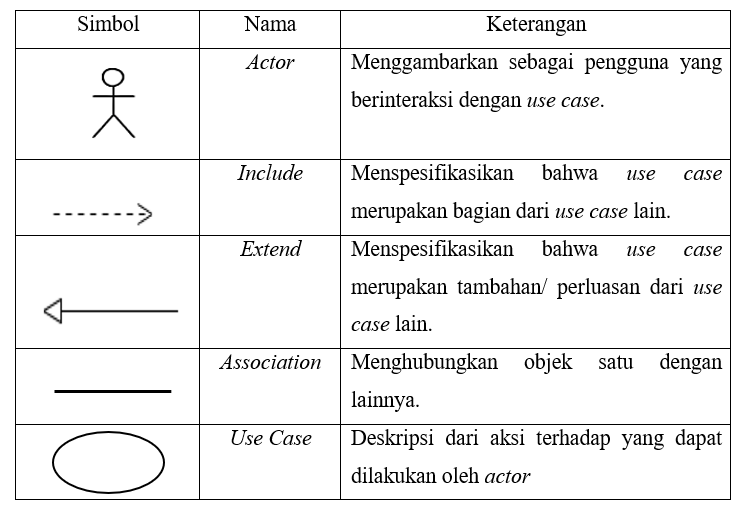
\includegraphics[width=1.0\textwidth]{gambar/simbolusecase}
	\label{tabel_karaktermax2}
\end{table}

\subsection{Diagram \emph{Class}} 

\emph{Class diagram} merupakan salah satu diagram utama dari UML untuk menggambarkan class atau \emph{blueprint object} pada sebuah sistem. Analisis pembentukan \emph{class diagram} merupakan aktivitas inti yang sangat memengaruhi arsitektur piranti lunak yang dirancang hingga ke tahap pengkodean \cite{tanuwijaya}.

%tabel Simbol Class Diagram
\begin{table}[H]
	\centering
	\caption{Simbol-simbol \emph{Class Diagram}}
	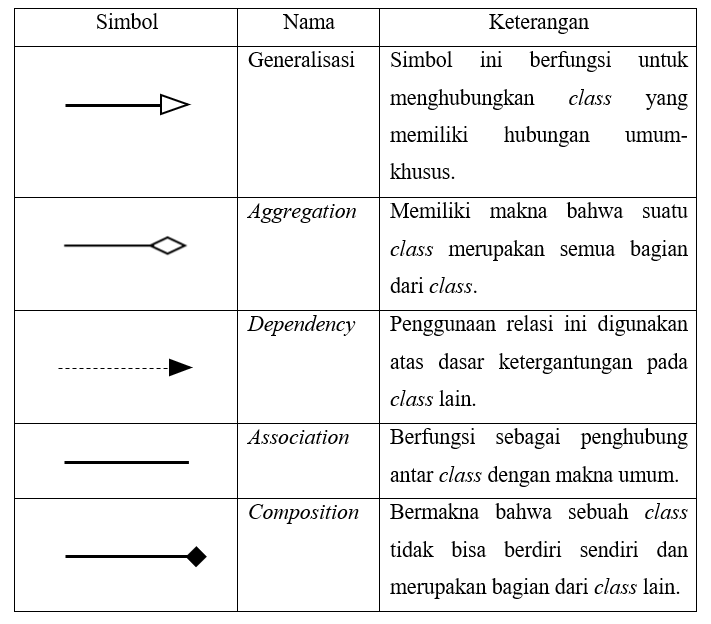
\includegraphics[width=1.0\textwidth]{gambar/simbolclass}
	\label{tabel_karaktermax2}
\end{table}

\subsection{Diagram \emph{Activity}} 

\emph{Activity diagram} menggambarkan berbagai alur kejadian dalam aktivitas sistem yang sedang dalam pengembangan, bagaimana masing-masing alur dimulai, kejadian yang mungkin terjadi, dan bagaimana mereka berakhir. Sebuah aktivitas dapat direalisasikan oleh satu \emph{use case} atau lebih. Aktivitas menggambarkan proses yang berjalan, sementara \emph{use case} menggambarkan bagaimana aktor menggunakan sistem untuk melakukan aktivitas.

%tabel Simbol Activity Diagram
\begin{table}[H]
	\centering
	\caption{Simbol-simbol \emph{Activity Diagram}}
	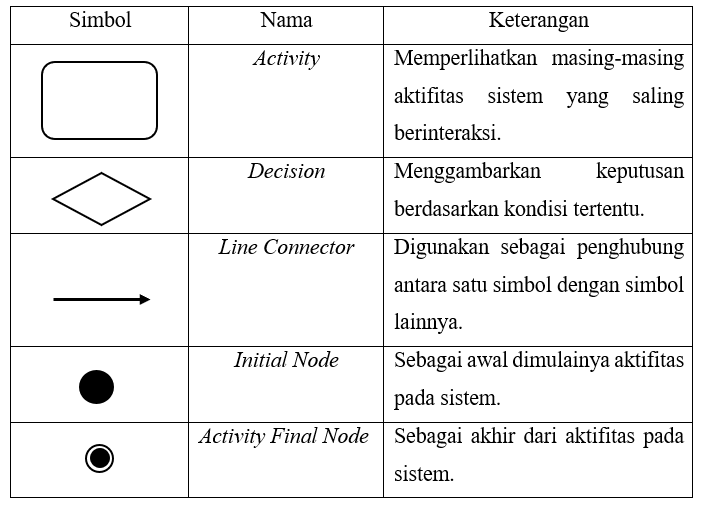
\includegraphics[width=1.0\textwidth]{gambar/simbolactivity}
	\label{tabel_karaktermax2}
\end{table}


\section{\emph{Entity Relationship Database}(ERD)}

ERD merupakan suatu model untuk menjelaskan hubungan antar data dalam \emph{database} berdasarkan objek-objek dasar data yang mempunyai hubungan antar relasi. ERD untuk memodelkan struktur data dan hubungan antar data, untuk menggambarkannya digunakan beberapa notasi dan simbol.

Menurut Brady serta Loonam (2010), \emph{Entity Relationship Diagram} (ERD) adalah suatu teknik yang digunakan untuk dapat memodelkan kebutuhan data dari sebuah organisasi. Biasanya dilakukan oleh \emph{system analys} di dalam tahap analisis persyaratan proyek pengembangan sistem \cite{ibeng}. 

Beberapa jenis relasi antar entitas yang ada pada ERD yaitu \emph{one-to-one}, \emph{one-to-many}, dan \emph{many-to-many}. Dari masing-masing relasi tersebut digunakan tergantung dari kebutuhan data antara entitas yang berhubungan. 

\section{Arsitektur \emph{Model View Controller} (MVC)}

Pola MVC memecah aplikasi menjadi 3 bagian yaitu \emph{model}, \emph{view}, \emph{controller}. Ketiga modul tersebut adalah inti dari aplikasi dan merupakan logika bisnisnya. MVC adalah sebuah konsep yang meng-enkapsulasi basis data, proses manipulasi, dan tampilan untuk direpresentasikan kepada pengguna \cite{simajuntak}. Definisi teknis dari MVC dibagi menjadi tiga bagian.

\subsection{Model}

\emph{Model} digunakan untuk mengolah informasi. Hanya model yang mengandung data dan fungsi yang berhubungan dengan pemrosesan data. Dengan kata lain, model adalah bagian yang mewakili struktur data dalam basis data.

\subsection{View}

\emph{View} adalah bagian yang berfungi dalam pemetaan grafis pada permukaan layar. Ketika ada perubahan dalam \emph{model}, maka \emph{view} akan secara otomatis me-\emph{render} kembali tampilan grafis dan menggambarkannya pada permukaan layar.

\subsection{Controller}

\emph{Controller} dapat disebut juga sebagai jembatan yang menghubungkan antara \emph{model} dan \emph{view}. \emph{Controller} bertanggung jawab dalam memanipulasi proses. Sebagai contoh ketika \emph{user} melakukan perintah \emph{input} maka \emph{controller} akan menentukan bagaimana aplikasi seharusnya merespon.

Secara singkat dapat disimpulkan bahwa \emph{model} bertanggung jawab dalam mengatur alur dari basis data, \emph{view} bertanggung jawab sebagai yang merepresentasikan hasil proses kepada \emph{user} melalui pemetaan pada tampilan layar, dan \emph{controller} bertanggung jawab sebagai penentu respon aplikasi terhadap \emph{input} yang diberikan oleh \emph{user}.

\section{\emph{Framework} Codeigniter} 

Codeigniter (CI) adalah sebuah \emph{framework}/ kerangka kerja aplikasi yang bekerja dibawah \emph{platform} PHP untuk mengembangkan program PHP dengan cara yang lebih sistematis. Codeigniter dikembangkan pertama kali oleh Rick Ellis dan menjadi kerangka kerja yang memiliki lisensi gratis untuk digunakan karena menggunakan lisensi \emph{open-source} apache/BSD dan gratis [7]. \textit{Programmer} tidak perlu melakukan pengembangan dari awal karena telah disediakan beberapa \emph{library} yang dapat digunakan untuk menyelesaikan berbagai permasalahan umum. Codeigniter sendiri menggunakan teknik \emph{Model View Controller} (MVC).

Adapun kelebihan yang dimiliki oleh codeigniter yang menjadi pertimbangan penulis dalam pengembangan penelitian ini antara lain \cite{yicheng} :

\begin{enumerate}
	\item Memiliki ukuran \emph{file} yang relatif kecil.
	\item Mudah dalam proses instalasi. 
	\item Tidak adanya aturan yang terlalu ketat dalam pengkodean.
	\item Mudah untuk migrasi dari satu \emph{server} ke \emph{server} lainnya.
	\item Mudah di-\emph{debug}.
	\item Koleksi \emph{library} yang dimiliki cukup banyak.
	\item Memiliki dokumentasi yang baik sehingga mudah untuk dipelajari.
\end{enumerate}

\section{XAMPP \emph{Server}}

XAMPP adalah sebuah perangkat lunak \emph{web server} Apache yang didalamnya sudah tersedia \emph{database server} MySQL dan mendukung bahasa pemrograman PHP. XAMPP merupakan singkatan dari X (untuk empat sistem operasi – windows, linux, macOS, dan solaris), Apache, MySQL, PHP, dan Perl \cite{binarso}.

\section{MySQL \emph{Database}}

MySQL merupakan salah satu \emph{software} sistem manajemen \emph{database} bersifat relasional yang disediakan secara gratis di bawah lisensi \emph{General Public License} (GPL). Bahasa SQL adalah bahasa yang menjadi standar bahasa untuk mengakses \emph{database} Oracle, SQL \emph{server}, DB2, dan MySQL \cite{andreea}. Perintah utama SQL terdiri dari lima kategori yaitu bahasa untuk melakukan permintaan, memanipulasi data, mendefinisikan data, kontrol transaksi, dan kontrol data. 

\section{Manajemen}

\subsection{Pengertian Manajemen}

Manajemen secara etimologi berasal dari bahasa inggris \emph{management} yang artinya mengatur atau mengelola. Sedangkan di dalam kamus besar bahasa Indonesia kata manajemen memiliki arti sebagai penggunaan sumber daya secara efektif untuk mencapai sasaran. Dalam arti khusus manajemen dipakai oleh pemimpin atau pimpinan yaitu orang-orang yang melakukan kegiatan memimpin didalam suatu organisasi \cite{syamsuddin}. 

Pada umumnya manajemen dikaitkan dengan kegiatan-kegiatan seperti perencanaan, pengorganisasian, pemberian, pengawasan, pengarahan dan menentukan keputusan. Dari penjelasan di atas dapat disimpulkan bahwa manajemen adalah kegiatan yang berkaitan dengan pengelolaan dengan cara memanfaatkan sumber daya secara efektif melalui beberapa tindakan perencanaan hingga pengambilan keputusan untuk mencapai tujuan dari suatu organisasi.

\subsection{Fungsi Manajemen}

Ada beberapa pendapat menurut para ahli mengenai fungsi dari manajemen adalah sebagai berikut \cite{rifai}: 

%tabel Pengertian Manajemen Menurut Ahli
\begin{table}[H]
	\centering
	\caption{Fungsi manajemen menurut para ahli}
	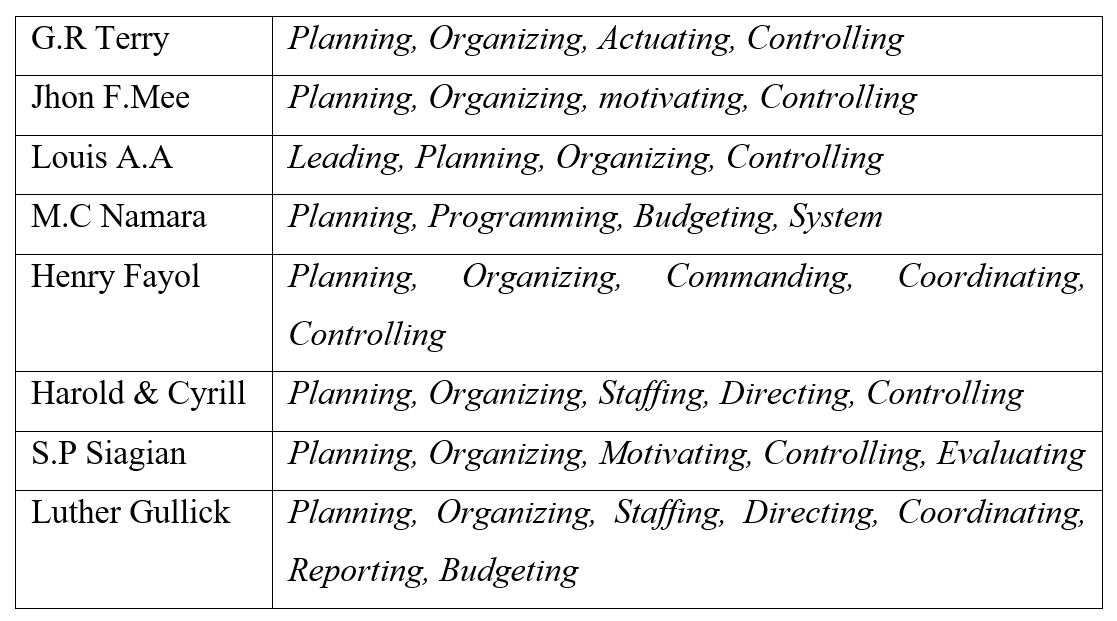
\includegraphics[width=1.0\textwidth]{gambar/manajemenmenurutahli}
	\label{tabel_karaktermax2}
\end{table}

Dari tabel di atas dapat disimpulkan bahwa ada empat fungsi yang menurut penulis penting yaitu perencanaan (\emph{planning}), pengorganisasian (\emph{organizing}), kepemimpinan (\emph{leading}), dan pengaturan (\emph{controlling}). Perencanaan merupakan kegiatan untuk memikirkan langkah kedepan untuk memberikan arah, meminimalisir pengulangan, dan mempermudah pengawasan. Pengorganisasian merupakan kegiatan pembatasan, pengelompokan, dan pemberian tugas kepada sumber daya manusia. Bagi seorang pemimpin organisasi kepemimpinan diperlukan untuk memanajemen sumber daya dan melakukan pengawasan atau pengaturan.

\subsection{Macam-macam Manajemen}

Manajemen dapat diterapkan didalam berbagai bentuk organisasi. Setiap organisasi memiliki norma dan aturan sendiri dalam menerapkan manajemen sebagai sistem yang menjalankan roda organisasi. Menurut Made Pidarta, sebuah sistem manajemen dapat dilihat dari berbagai sudut pandang berikut \cite{athhoillah} :

\begin{enumerate}
	\item \emph{Management by objective} \\*
	Dalam manajemen sasaran, seluruh elemen diintegrasikan dan ditargetkan kepada sasaran atau tujuan yang telah ditentukan. Biasanya dalam organisasi memiliki tiga tingkatan, yaitu tujuan jangka pendek, tujuan jangka menengah, dan tujuan jangka panjang. Manajemen berdasarkan sasaran sangat mementingkan adaptabilitas semua subsistem dan komponen di dalamnya. Dalam pelaksanaan rencana kegiatan interaktif adaptif antara tujuan dan seluruh sumber daya. Dengan demikian seluruh komponen di dalam organisasi harus memiliki ikatan yang kuat untuk mewujudkan tujuannya. 
	
	\item \emph{Management by structures} \\*
	Manajemen dengan pendekatan struktural berawal dari pandangan bahwa organisasi adalah struktur yang harus dikelola secara struktural. Oleh karena itu pelaksanaan manajerial berdasarkan kedudukan, peran, dan tugas setiap personalia dalam strukturnya masing-masing.
	
	\item \emph{Management by technique} \\*
	Dalam manajemen Teknik, penguasaan terhadap Teknik-teknik pelaksanaan kegiatan lebih diutamakan. Sebagai contoh, sebuah organisasi menginginkan sebuah acara yang menggabungkan suasana tradisional namun tetap bernuansa modern. Hal-hal yang dibahas lebih tertuju kepada bagaimana cara perpaduan yang dimaksud, apa saja alat yang diperlukan, berapa biayanya, dan hal-hal teknis lainnya.
	
	\item \emph{Management by people} \\*
	Manajemen ini mengutamakan sumber daya manusia sebagai pelaksana seluruh rencana organisasi. Orang-orang yang terlibat disebut sebagai personalia. Dalam manajemen personalia, seorang pimpinan tertinggi tidak hanya terpaku pada hubungan vertikal kekuasaan struktural, tetapi perlu juga membangun hubungan yang interaktif dengan seluruh bawahannya.
	
	\item \emph{Management by information} \\*
	Manajemen dengan pendekatan informasi adalah pengelolaan organisasi yang berpusat pada peran pentingnya informasi bagi kemajuan dan kinerja organisasi. Informasi merupakan media yang menciptakan relasi maupun sebagai data untuk mengetahui keadaan organisasi yang sesungguhnya. Informasi bukan hanya menjadi sebuah berita, melainkan tentang berbagai kondisi internal maupun eksternal organisasi.
	
	\item \emph{Management by environment} \\*
	Lingkungan organisasi adalah segala sesuatu yang ada di sekeliling organisasi. Faktor internal dan eksternal seperti manusia, fasilitas, sarana, transportasi dan lain-lain. Lingkungan yang sangat menentukan kemajuan organisasi adalah lingkungan masyarakat karena organisasi mengadakan kontak secara langsung dengan masyarakat. Contohnya, pertokoan yang dekat dengan organisasi akan lebih memudahkan organisasi dalam memeroleh barang yang dibutuhkan.
\end{enumerate}

\section{Program Kerja}

Program kerja adalah sebuah susunan rencana kegiatan yang telah dirancang dan disepakati bersama oleh anggota/ pengurus organisasi untuk dilaksanakan dalam jangka waktu tertentu. Program kerja bertujuan sebagai media untuk merealisasikan visi dan misi dari organisasi, membantu menjawab kebutuhan organisasi baik dari segi internal maupun eksternal, dan membantu organisasi bekerja secara sistematis dan terstruktur \cite{dosen}.

Program kerja yang ada di opmawa pada umumnya terdiri dari dua jenis program kerja yaitu program kerja yang bersifat \emph{event} dan program kerja yang bersifat \emph{non-event}. Program kerja \emph{event} merupakan kegiatan yang melibatkan masyarakat umum di dalam pelaksanaannya. Contoh dari program kerja  yang bersifat \emph{event} antara lain berupa seminar, \emph{workshop}, dan sebagainya. Sedangkan program kerja \emph{non-event} biasanya hanya bersifat internal dalam organisasi untuk meningkatkan kebersamaan dan kemampuan berorganisasi.

Adapun tahapan-tahapan dalam pelaksanaan program kerja secara umum antara lain yaitu studi kasus permasalahan dan kebutuhan, perencanaan kegiatan, pelaksanaan, dan evaluasi.

\section{Penelitian Relevan}
Beberapa hasil penelitian mengenai sistem informasi manajemen yang relevan sebelumnya dengan penelitian ini antara lain:

\begin{enumerate}[A.]
	\item Penelitian yang dilakukan oleh Yogi Perdana pada tahun 2019 dalam skripsinya yang berjudul “Perancangan dan Implementasi Aplikasi Penilaian Kinerja Badan Eksekutif Mahasiswa Universitas Negeri Jakarta Berbasis \emph{Web}”. Model pengembangan perangkat lunak yang digunakan adalah dengan menggunakan model Spiral. Penelitian tersebut bertujuan untuk memberikan penilaian terhadap kinerja Badan Eksekutif Mahasiswa (BEM) melalui instrumen penilaian yang telah ditetapkan oleh Badan Legislatif Mahasiswa atau biasa disebut sebagai Majelis Tinggi Mahasiswa (MTM) terhadap program kerja BEM yang telah terlaksana. Sistem tersebut memungkinkan MTM untuk mengelola instrumen penilaian sebagai acuan untuk penilaian kinerja BEM dengan cara membuat indikator penilaian beserta bobot untuk setiap indikatornya. Setelah instrumen penilaian telah ditetapkan, maka komisi yang berkaitan memberikan penilaian terhadap program kerja BEM sesuai dengan interval bobot untuk setiap indikator penilaian \cite{perdana}.
	
	Persamaan penelitian tersebut dengan penelitian yang akan penulis lakukan adalah sama-sama berkaitan dengan program kerja yang di lakukan oleh BEM. Model pengembangan yang digunakan sama-sama menggunakan model Spiral dan menggunakan \emph{framework} yang sama yaitu Codeigniter. Pada penelitian ini, sistem yang akan dibangun juga dapat memberikan penilaian terhadap program kerja BEM yang telah terlaksana.
	
	Perbedaannya dalam penelitian tersebut dengan penelitian yang akan penulis lakukan terletak pada fokus dan tingkatan opmawa. Penelitian tersebut terfokus pada pembuatan instrumen penilaian, sedangkan penelitian yang akan penulis lakukan terfokus pada proses manajemen program kerja dari awal terencananya program kerja hingga program kerja tersebut selesai terlaksana. Pada penelitian ini juga memungkinkan sebagai jembatan informasi antar lintas lembaga dan lintas periode kepengurusan opmawa. Pada penelitian tersebut bertujuan untuk opmawa pada tingkat Universitas sedangkan penelitian ini berada pada opmawa tingkat Fakultas.
	
	\item Penelitian yang dilakukan oleh Muhammad Yan Handoko pada tahun 2019 dalam skripsinya yang berjudul "Perancangan Sistem Informasi Koperasi Serba Usaha Berbasis \textit{Website} Pada Lembaga Koperasi Mahasiswa Universitas Negeri Jakarta". Model pengembangan perangkat lunak yang digunakan adalah dengan menggunakan model Spiral. Penelitian tersebut bertujuan untuk membangun sistem informasi yang dapat mempermudah pengolahan data baik itu pengolahan data anggota, simpanan, usaha, dan pendistribusian sisa hasil usaha \cite{handoko}. 
	
	Persamaan penelitian tersebut dengan penelitian yang akan penulis lakukan adalah sama-sama berkaitan dengan fungsi manajerial organisasi dalam menjalankan program kerjanya dan menggunakan model pengembangan Spiral. Kedua sistem juga dikembangkan menggunakan \textit{framework} yang sama.
	
	Perbedaannya dalam penelitian tersebut dengan penelitian yang akan penulis lakukan terletak pada organisasi yang menjadi objek penelitian dan perbedaan program kerja yang dilaksanakan oleh masing-masing organisasi.
	
	\item Penelitian yang dilakukan oleh La Ode Ismail Ahmad dan Ristati Sinen dalam jurnal Idaarah Vol.I No.2 Desember 2017 menjelaskan tentang penerapan sistem informasi manajemen pada SMPN 21 Makassar. Penggunaan sistem informasi manajemen pada dunia pendidikan diperlukan guna meningkatkan efesiensi dalam kegiatan belajar mengajar dan memberikan kesempatan kepada guru dan pengurus sekolah untuk meningkatkan kualitas komunikasi dan pembinaan kepada siswa \cite{ahmad}.
	
	Persamaan penelitian tersebut dengan penelitian yang akan penulis lakukan adalah pemanfaatan sistem informasi manajemen dalam pengolahan data untuk diolah menjadi sebuah informasi yang berguna dalam pengambilan keputusan manajerial. Sistem yang akan dirancang oleh penulis memiliki tujuan yang sama dengan sistem informasi manajemen yang ada pada SMPN 21 Makassar. 
 
 	Perbedaannya dalam penelitian tersebut dengan penelitian yang akan penulis lakukan terletak pada objek organisasi dan pokok pembahasan yang diteliti.
 	
 	\item Penelitian yang dilakukan oleh Etin Indrayani dalam \textit{Journal of Social Sciences Research} Vol.9 No.3 Desember 2015 menjelaskan tentang pengimplementasian sistem informasi manajemen pada pelayanan administrasi kecamatan Sragen. Pada penelitian tersebut membahas mengenai penggunaan sistem informasi manajemen dalam mengoperasikan fungsional organisasi \cite{indrayani}.
 	
 	Persamaan penelitian tersebut dengan penelitian yang akan penulis lakukan adalah pembahasan mengenai pemanfaatan sistem informasi manajemen dalam pengelolaan fungsional organisasi. Pengelolaan terkait pada permasalahan anggaran, keanggotaan, penyebaran informasi, interaksi organisasi eksekutif, dan lain-lain.
 	
 	Perbedaannya dalam penelitian tersebut dengan penelitian yang akan penulis lakukan terletak pada objek organisasi dan pokok pembahasan yang diteliti.
	
	
\end{enumerate}

		
% Baris ini digunakan untuk membantu dalam melakukan sitasi
% Karena diapit dengan comment, maka baris ini akan diabaikan
% oleh compiler LaTeX.
\begin{comment}
bibliography{daftar-pustaka}
\end{comment}


%!TEX root = ./template-skripsi.tex
%-------------------------------------------------------------------------------
%                            BAB III
%               			PEMBAHASAN
%-------------------------------------------------------------------------------

\chapter{IMPLEMENTASI PROGRAM}

Dalam mengembangkan perangkat lunak ini, penulis menggunakan model Spiral seperti yang telah tertera pada \emph{System Development Life Cycle}. Tahapan-tahapannya antara lain adalah identifikasi masalah, pembangunan rancangan (desain), implementasi kode, dan evaluasi sistem.



\section{Identifikasi Masalah}

Penulis melakukan wawancara dengan perwakilan opmawa pada tanggal 22 April 2019 dan pada tanggal 20 Mei 2019. Dari hasil wawancara tersebut diperoleh hasil sebagai berikut: 

\begin{enumerate}
	\item Penyebaran informasi mengenai segala bentuk kegiatan atau program kerja dilakukan di media sosial Whatsapp, Instagram, dan Line.
	
	\item Berkas pada umumnya disimpan di penyimpanan internal gawai anggota yang bersangkutan.
\end{enumerate}

Dari wawancara yang telah dilakukan, ditemukan beberapa kendala yang sering dialami oleh opmawa selama proses pelaksanaan program kerja. Kendala-kendala tersebut antara lain:

\begin{enumerate}
	\item Informasi penting melalui pesan hilang karena pesan yang diberikan telah tertimbun oleh pesan lainnya.
	
	\item Pengarsipan dokumen yang belum baik sehingga memengaruhi kinerja pelaksanaan program kerja.
	
	\item Terjadinya \emph{miss communication} jika ada agenda untuk melakukan kumpul/ rapat bersama.
	
	\item Beberapa anggota ada yang tidak/ kurang mengetahui rencana program kerja yang telah di rencanakan beserta prosesnya.
	
	\item Anggota kepengurusan periode saat ini, ada yang tidak mengetahui mengenai pencapaian/ evaluasi dari tahun kepengurusan periode sebelumnya.
\end{enumerate}

Bersadarkan permasalahan tersebut penulis memberikan usulan mengenai perangkat lunak yang akan dikembangkan antara lain:

\begin{enumerate}
	\item Aplikasi dibuat dengan dua \emph{user} yaitu Badan Eksekutif Mahasiswa (BEM) dan Badan Perwakilan Mahasiswa (BPM).
	
	\item BEM dapat mengelola hal-hal yang berkaitan dengan pelaksanaan program kerja maupun pendaftaran kabinet kepengurusan.
	
	\item BPM dapat mengelola program kerja yang dilakukan oleh BPM dan dapat memberikan penilaian terhadap program kerja yang dilakukan oleh BEM.
\end{enumerate}

\section{Pembangunan Perancangan (Desain)}

Pada tahap ini penulis akan merepresentasikan gambaran dan kebutuhan sistem melalui bentuk komunikasi visual berupa \emph{use case diagram}, \emph{entity relationship database}, \emph{activity diagram}, dan \emph{user interface}.

\subsection{Diagram \emph{Use Case}}
\emph{User} pada aplikasi ini terdiri dari dua lembaga yaitu Badan Eksekutif Mahasiswa (BEM) dan Badan Perwakilan Mahasiswa (BPM). Adapun hal-hal yang dapat dilakukan oleh BEM antara lain:

\begin{enumerate}
	\item Mengubah profil BEM.
	\item Kelola registrasi sistem (prodi, jabatan, kabinet).
	\item Kelola keanggotaan BEM.
	\item Kelola program kerja BEM.
	\item Kelola kepanitiaan program kerja.
	\item Kelola berkas BEM.
	\item Kelola pembagian tugas dalam program kerja.
	\item Kelola keuangan. 
	\item Kelola evaluasi program kerja.
	\item Kelola agenda rapat.	
\end{enumerate}

Berikut adalah hal-hal yang dapat dilakukan oleh BPM antara lain:

\begin{enumerate}
	\item Mengubah profil BPM.
	\item Kelola keanggotaan BPM.
	\item Kelola program kerja BPM.
	\item Kelola anggota komisi pada divisi/ departemen yang didaftarkan oleh BEM.
	\item Kelola berkas BPM.
	\item Kelola agenda rapat.
	\item Mengisi penilaian pada program kerja yang dilaksanakan oleh BEM.
	Mengisi evaluasi program kerja untuk program kerja BEM.
\end{enumerate}

Berikut adalah \emph{use case diagram} yang dapat digambarkan dari berbagai fitur yang telah disebutkan dari aplikasi sistem informasi manajemen program kerja :

\begin{figure}[H]
	\centering
	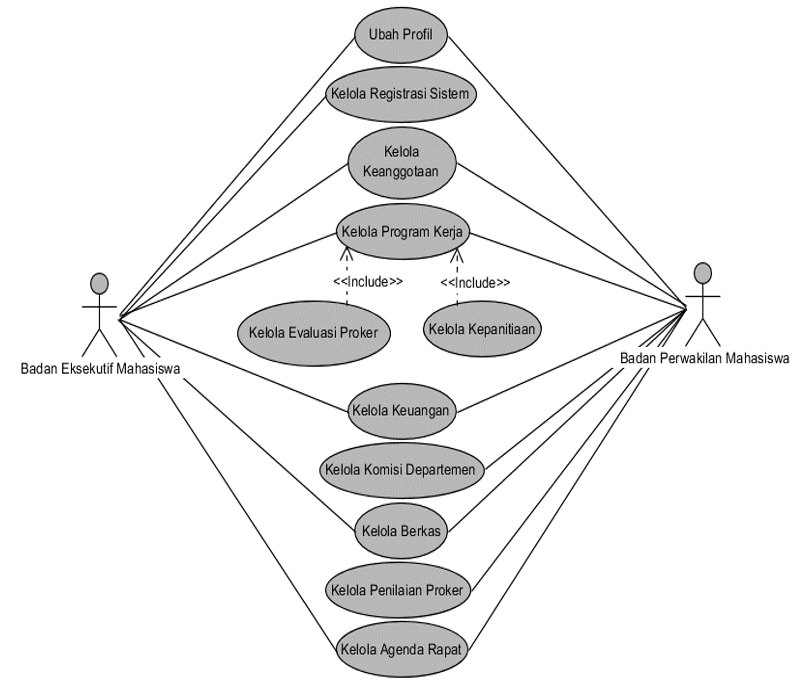
\includegraphics[width=1.0\textwidth]{gambar/usecase}
	\caption{Desain \emph{Use Case Diagram} Sistem Informasi Manajemen}
	\label{usecase_diagram}
\end{figure}

Pada sistem ini, BEM dapat mengelola data registrasi pada sistem seperti data mengenai daftar Program Studi dan daftar nama departemen yang ada pada periode kepengurusan. Sedangkan BPM dapat mengelola program kerja dan memberikan penilaian terhadap program kerja BEM yang telah terlaksana.

\subsection{\emph{Entity Relationship Diagram}}

ERD pada aplikasi ini berfungsi sebagai gambaran desain \emph{database} beserta relasi-relasi antar tabel. Penulis membuat desain \textit{database} yang terdiri dari 14 (empat belas) tabel yang saling berintegrasi. Tabel-tabel tersebut digunakan untuk menyimpan data mengenai data \textit{user}, keuangan, program kerja, kepanitiaan, pemberkasan, dan agenda rapat.

\begin{figure}[H]
	\centering
	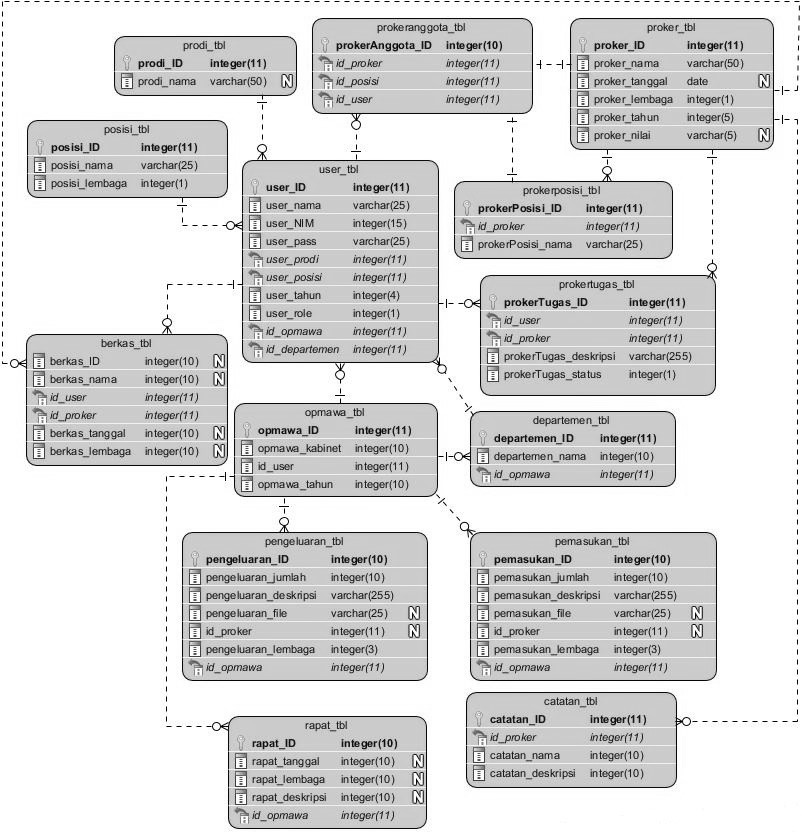
\includegraphics[width=1.0\textwidth]{gambar/erd}
	\caption{Desain \emph{Entity Relationship Diagram} Sistem Informasi Manajemen}
	\label{entityrelationship_diagram}
\end{figure}

\subsection{\textit{Class Diagram}}

\textit{Class diagram} pada aplikasi sistem informasi manajemen program kerja terdiri dari 10 (sepuluh) \textit{class} yang saling terhubung. \textit{Class user} yang menyimpan metode untuk \textit{login} atau \textit{logout}. \textit{Class user} merupakan generalisasi dari dua \textit{class} lainnya yaitu \textit{class} Badan Legislatif dan \textit{class} Badan Eksekutif. \textit{Class} program kerja berfungsi untuk menyimpan metode pendataan program kerja. \textit{Class} kepanitiaan merupakan \textit{class} yang tidak dapat berdiri sendiri tanpa adanya \textit{class} program kerja. \textit{Class} lembaga merupakan bagian dari \textit{class user} dan program kerja. \textit{Class} berkas, catatan, dan keuangan memiliki relasi dengan \textit{class} lembaga dan adakalanya dibutuhkan oleh \textit{class} program kerja. Dan yang terakhir adalah \textit{class} jadwal rapat yang berfungsi sebagai jadwal agenda rapat oleh \textit{user}.

\begin{figure}[H]
	\centering
	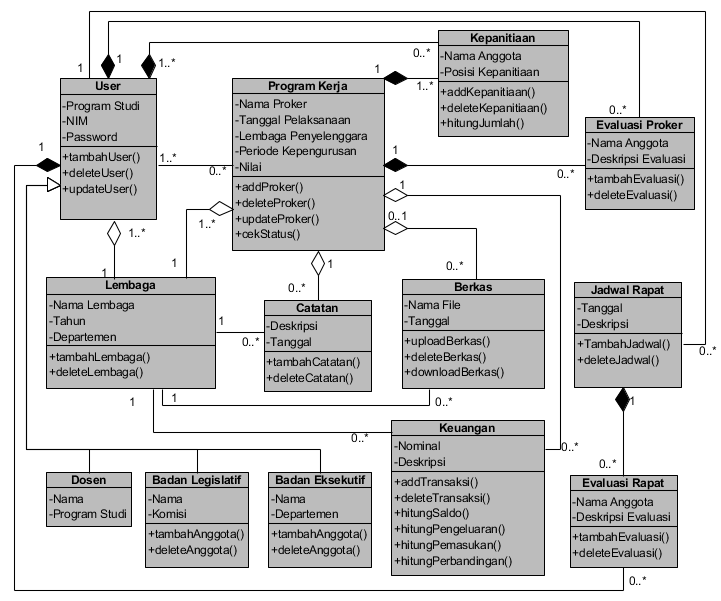
\includegraphics[width=1.0\textwidth]{gambar/after_sps/classv2}
	\caption{Desain \emph{Class Diagram} Sistem Informasi Manajemen}
	\label{class_diagram}
\end{figure}


\subsection{\textit{Activity Diagram}}

\textit{Activity diagram} pada aplikasi sistem informasi manajemen program kerja opmawa meliputi alur pendaftaran anggota, pendaftaran program kerja dan kepanitiaannya, pencatatan keuangan program kerja/ umum, dan registrasi sistem. Berikut gambaran beberapa desain visual untuk \textit{activity diagram} aplikasi sistem informasi manajemen program kerja :

\begin{figure}[H]
	\centering
	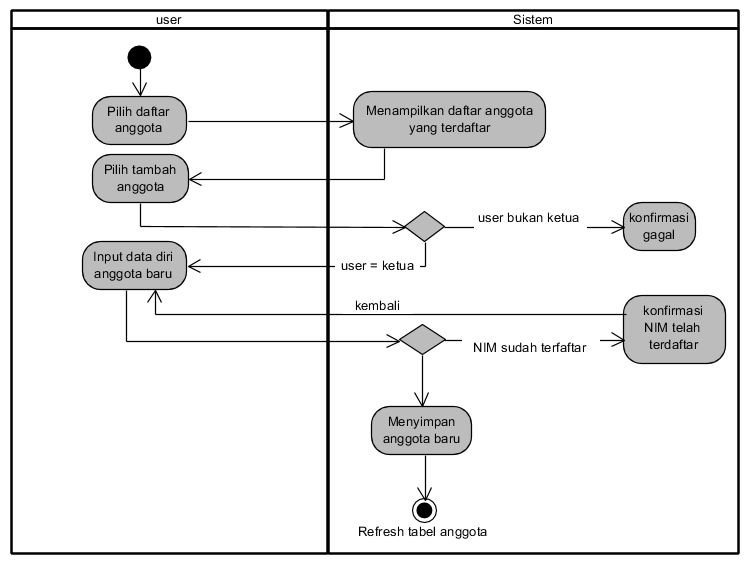
\includegraphics[width=1.0\textwidth]{gambar/Activitytambahanggota}
	\caption{Desain \emph{Activity Diagram} Pendaftaran Anggota}
	\label{activityAnggota_diagram}
\end{figure}

Pada alur pendaftaran anggota, hanya ketua dari masing-masing lembaga (eksekutif/ legislatif) yang dapat mendaftarkan anggota nya. Ketua mendaftarkan anggota baru dengan mengisi \textit{form} pendaftaran, kemudian sistem akan melakukan pemeriksaan. Apabila NIM (Nomor Induk Mahasiswa) sudah terdaftar dan NIM yang terdaftar tersebut memiliki data periode kepanitiaan yang sama dengan ketua, maka sistem akan otomatis menolak dan mengarahkan untuk mengisi ulang \textit{form}. Jika NIM belum terdaftar, maka data akan tersimpan dalam \textit{database}.


\begin{figure}[H]
	\centering
	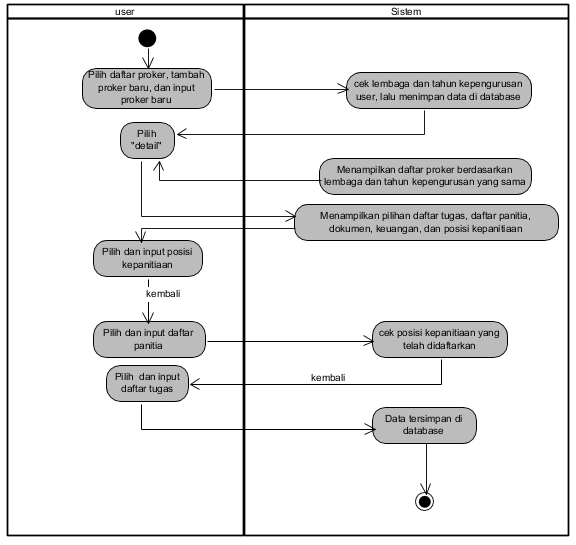
\includegraphics[width=1.0\textwidth]{gambar/Activityproker}
	\caption{Desain \textit{Activity Diagram} Pendaftaran Program Kerja Dan Kepanitiaannya}
	\label{activityProker_diagram}
\end{figure}

Pada alur pendaftaran program kerja dan kepanitiaannya, \textit{user} meng-\textit{input} nama program kerja beserta rencana tanggal pelaksanaannya. Pada kolom tanggal dapat dikosongkan terlebih dahulu. Setelah mengisi \textit{form}, sistem akan mengambil beberapa data dari \textit{user} untuk mengklasifikasikan program kerja berdasarkan periode kepengurusan dan lembaganya. Setelah berhasil, \textit{user} dapat memilih secara bebas untuk mengelola data dari program kerja. 

\textit{User} dapat terlebih dahulu mendaftarkan posisi kepanitiaan yang diinginkan, kemudian mendaftarkan masing-masing anggota untuk masuk kedalam kepanitiaan dengan posisi kepanitiaan seperti yang telah terdaftar. Setelah data tersimpan, selanjutnya \textit{user} dapat mengelola data-data lainnya seperti catatan mengenai program kerja, keuangan, unduh/ unggah dokumen, dan memberikan catatan penugasan untuk setiap anggota kepanitiaan. 

\begin{figure}[H]
	\centering
	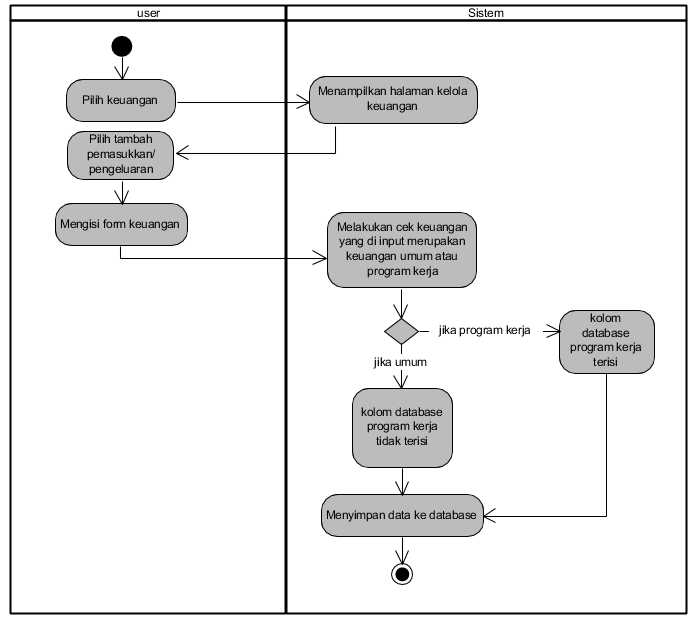
\includegraphics[width=1.0\textwidth]{gambar/Activitykeuangan}
	\caption{Desain \textit{Activity Diagram} Kelola Keuangan}
	\label{ActivityKeuangan_diagram}
\end{figure}

Alur keuangan terbagi atas 2 jenis kelola keuangan yaitu kelola keuangan umum dan kelola keuangan yang berkaitan dengan pelaksanaan program kerja. \textit{User} dapat mengelola keuangan melalui \textit{menu side bar} untuk mengelola keuangan umum/ program kerja dan pada halaman detail program kerja untuk mengelola keuangan program kerja.

\begin{figure}[H]
	\centering
	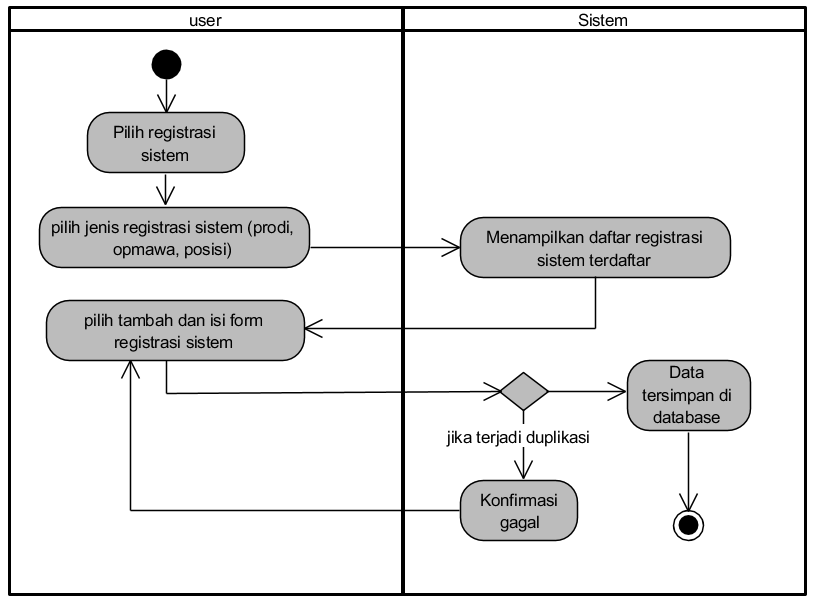
\includegraphics[width=1.0\textwidth]{gambar/Activitysistem}
	\caption{Desain \textit{Activity Diagram} Registrasi Sistem}
	\label{ActivitySistem_diagram}
\end{figure}

Registrasi sistem terdiri dari 3 jenis yaitu registrasi Program Studi, registrasi opmawa, dan registrasi posisi. Registrasi ini sebagai salah satu sekaligus pelengkap parameter \textit{input} pada \textit{form} yang membutuhkan data tertentu.

Registrasi Program Studi untuk mendaftarkan Program Studi yang ada di FMIPA, registrasi opmawa untuk mendaftarkan periode kepengurusan opmawa berikutnya, dan registrasi posisi untuk menentukan posisi-posisi atau struktur organisasi yang diperlukan dalam menjalani organisasi di opmawa.


\subsection{Desain \textit{Interface}}

Pada tampilan awal \textit{login} sebagai anggota BEM, terdapat pilihan untuk mendaftarkan anggota, daftar program kerja, kelola keuangan, kelola berkas/ dokumen, daftar agenda rapat, dan registrasi sistem. Berikut adalah desain untuk tampilan pada halaman BEM :

\begin{figure}[H]
	\centering
	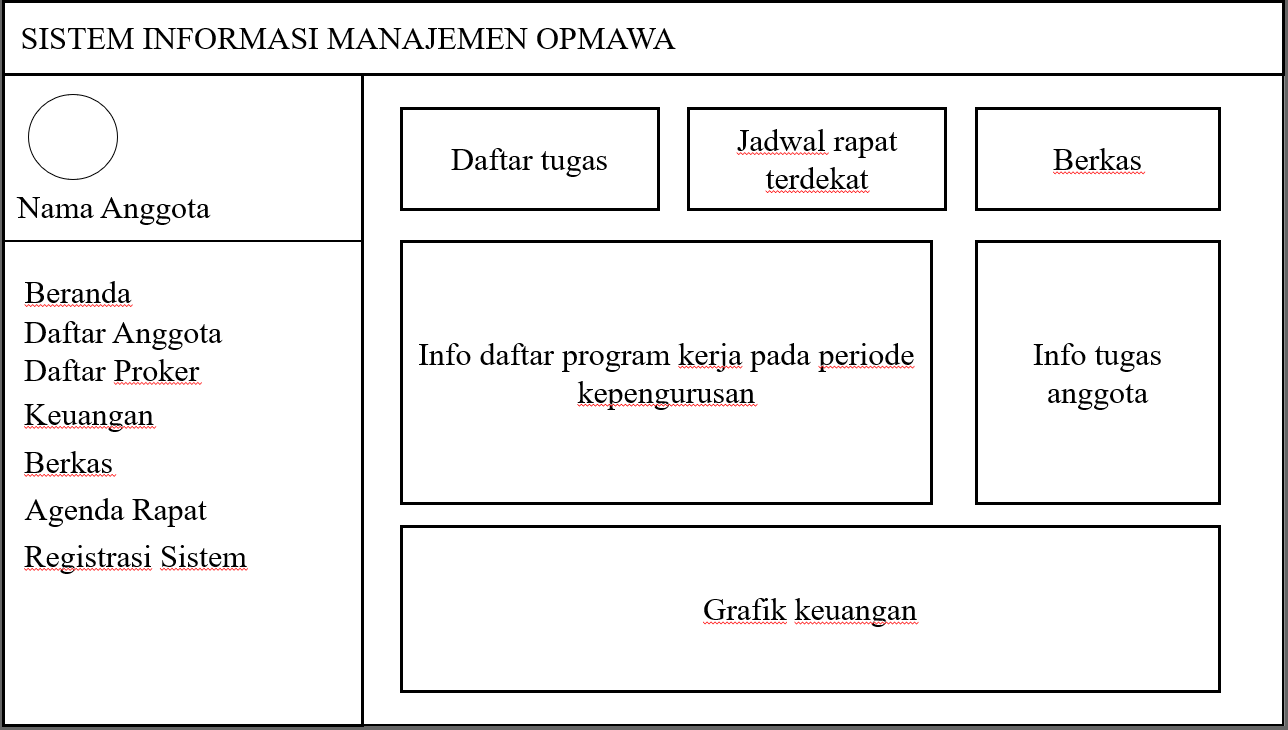
\includegraphics[width=0.9\textwidth]{gambar/tampilanberanda}
	\caption{Desain Tampilan Awal / Beranda}
	\label{Tampilan_beranda}
\end{figure}

Gambar 3.8 menampilkan gambaran desain untuk tampilan setelah \textit{login} sebagai anggota BEM. Pada tampilan awal ini, \textit{user} dapat melihat daftar pilihan dan tampilan informasi seperti daftar tugas, informasi mengenai program kerja yang akan dilaksanakan pada periode kepengurusan yang sesuai dengan \textit{user}, info tugas yang diberikan oleh \textit{user}, dan grafik keuangan yang di bagi berdasarkan pemasukan dan pengeluaran dari masing-masing program kerja yang telah terdaftar.


\begin{figure}[H]
	\centering
	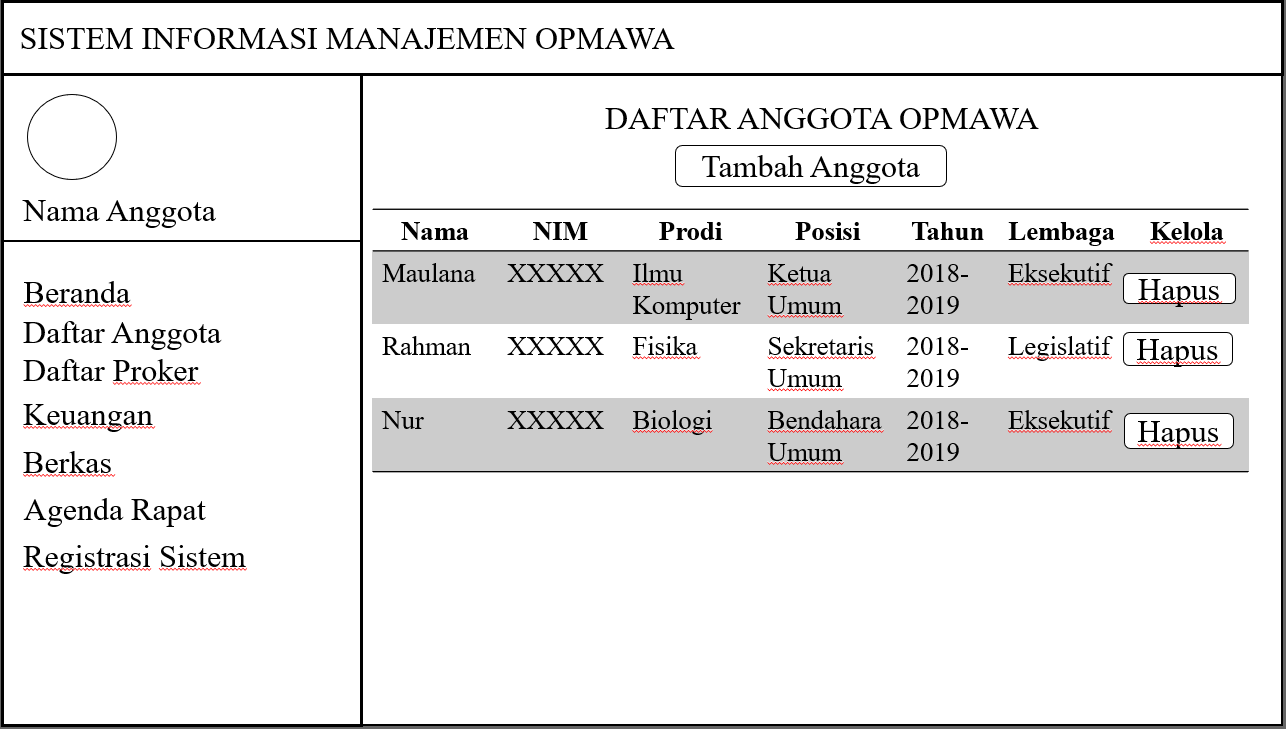
\includegraphics[width=0.9\textwidth]{gambar/tampilananggota}
	\caption{Desain Tampilan Daftar Anggota opmawa}
	\label{Tampilan_anggota}
\end{figure}

Gambar 3.9 merupakan desain tampilan daftar anggota yang telah terdaftar untuk periode kepengurusan tertentu. Di tampilan ini, \textit{user} yang berada pada posisi ketua lembaga juga memungkinkan untuk mendaftarkan anggota baru atau menghapus anggota lama. Ketua lembaga hanya dapat mengelola daftar anggota yang berada pada lembaga yang sama.

\begin{figure}[H]
	\centering
	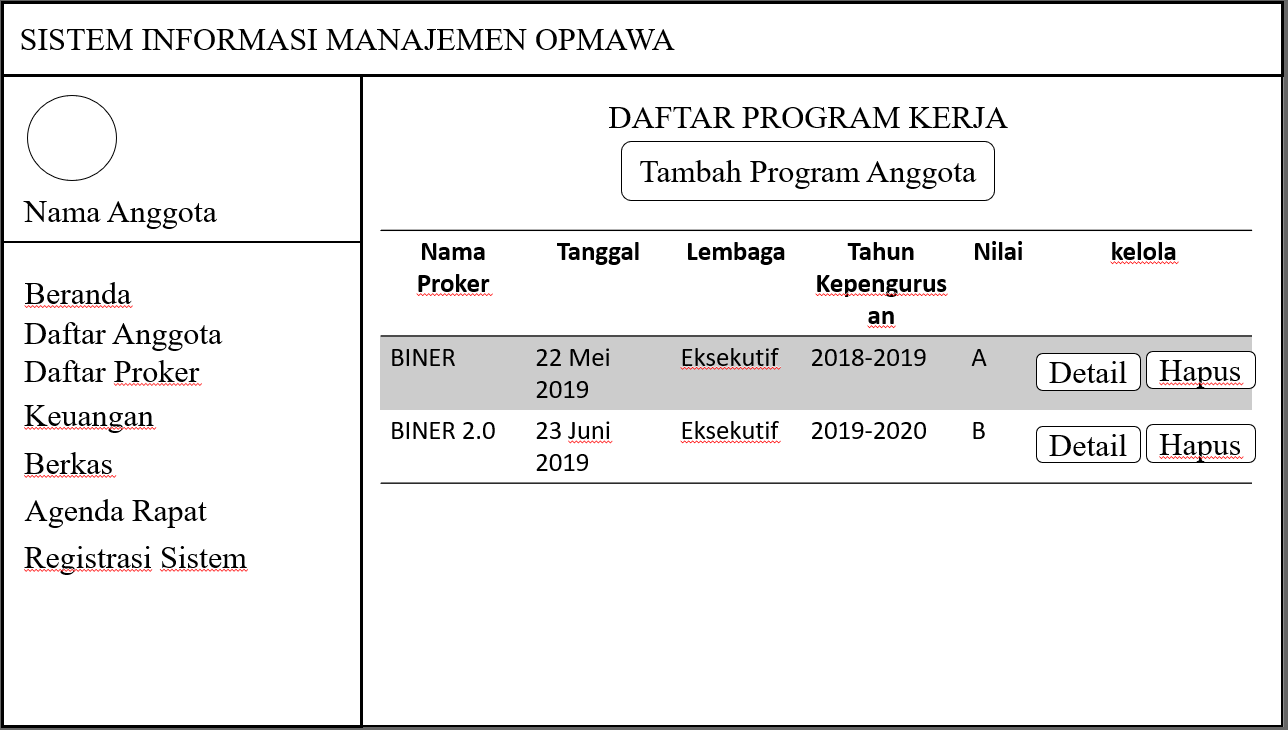
\includegraphics[width=0.9\textwidth]{gambar/tampilanproker}
	\caption{Desain Tampilan Daftar Program Kerja}
	\label{Tampilan_proker}
\end{figure}

Gambar 3.10 merupakan desain tampilan daftar program kerja yang telah direncanakan dan didaftarkan pada periode yang sesuai dengan tahun kepengurusan \textit{user} yang mendaftarkannya. \textit{User} juga dapat melihat informasi lebih mengenai program kerja dengan memilih opsi detail. Pada kolom "Nilai" hanya akan terisi apabila tanggal pelaksanaan program kerja telah terlewati dan diisi oleh lembaga legislatif.

\begin{figure}[H]
	\centering
	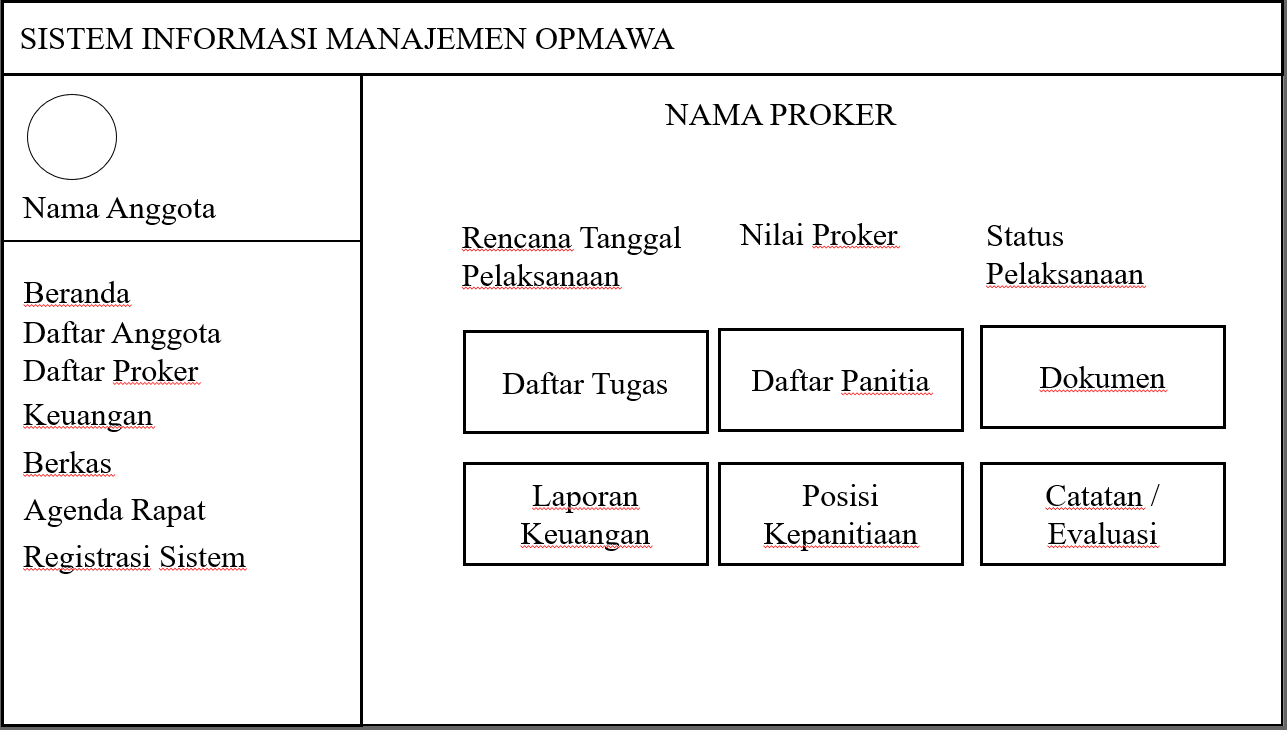
\includegraphics[width=0.9\textwidth]{gambar/tampilandetailproker}
	\caption{Desain Tampilan Detail Program Kerja}
	\label{Tampilan_detail_proker}
\end{figure}

Gambar 3.11 merupakan desain tampilan detail program kerja yang terdaftar. Pada tampilan ini memungkinkan \textit{user} untuk melihat tanggal pelaksanaan dan penilaian program kerja apabila telah selesai terlaksana, mengelola data-data dan keperluan lainnya pada suatu program kerja seperti mendaftarkan posisi kepanitiaan, mendaftarkan anggota opmawa yang akan terlibat dalam kepanitiaan, laporan keuangan, daftar-daftar tugas atau hal yang perlu dilakukan saat menjalankan program kerja, unduh atau unggah dokumen, dan catatan-catatan lainnya yang sekiranya diperlukan sebagai catatan maupun evaluasi yang terjadi dalam pelaksanaan program kerja.

\addcontentsline{toc}{chapter}{DAFTAR PUSTAKA}

%%!TEX root = ./template-skripsi.tex
%-------------------------------------------------------------------------------
%                            	BAB IV
%               		KESIMPULAN DAN SARAN
%-------------------------------------------------------------------------------

\chapter{UJI COBA DAN HASIL UJI COBA}

\section{Uji Coba}
Berdasarkan tahapan pengembangan pada metode spiral, setelah melakukan tahap implementasi/pengembangan terdapat tahapan selanjutnya yaitu tahapan evaluasi. Dalam tahapan ini penulis melakukan evaluasi dengan total 5 orang responden. Dari kelima orang responden terdiri dari 1 responden sebagai \textit{user} dosen, 2 orang sebagai perwakilan \textit{user} Lembaga Legislatif, dan 2 orang sebagai perwakilan \textit{user} Lembaga Eksekutif.

Penulis melakukan evaluasi dengan menggunakan kuisioner yang akan diberikan kepada masing-masing responden yang biasa disebut sebagai \textit{user acceptance test}. Pengujian ini bertujuan untuk mengetahui apakah sistem yang dikembangkan sudah dapat berjalan dengan baik sesuai fungsi dan kebutuhannya. Berikut adalah langkah-langkah pengujian aplikasi sistem informasi manajemen program kerja:

\begin{enumerate}
	\item Format \emph{file} citra yang bisa digunakan adalah format *.bmp 24 bit dan 32 bit karena mengandung RGB (\emph{Red, Green, Blue}), sedangkan pada \emph{file} citra 8 bit tidak dapat diproses karena tidak mengandung RGB.
	
	\item Pesan dalam format teks berhasil untuk disisipkan ke dalam \emph{file} citra dengan syarat tidak melebihi kapasitas maksimal dari \emph{file} citra tersebut.
	
	\item \emph{File} citra yang digunakan baik sebelum dan sesudah diproses tidak berubah. Perubahan yang terjadi tidak dapat dilihat secara visual.
	
	\item Pesan dalam \emph{Stego Image} dapat ditampilkan kembali dan sesuai dengan pesan awal. Kecuali ketika \emph{Stego Image} di-\emph{crop} maka pesan asli yang terdapat di \emph{file} citra tersebut tidak dapat ditampilkan kembali.

\end{enumerate}


\section{Saran}
Adapun saran-saran penulis untuk penelitian selanjutnya adalah:
\begin{enumerate}
	\item Program ini hanya dapat menyisipkan pesan berupa teks, diharapkan untuk kedepannya dikembangkan sehingga dapat menyisipkan \emph{file}, gambar atau audio.
	
	\item Media yang digunakan berupa \emph{file} citra, diharapkan dapat menggunakan media lain seperti audio.
	
	\item Program steganografi ini masih dikembangkan dengan MATLAB untuk perangkat komputer, diharapkan dapat dikembangkan lebih lanjut untuk perangkat \emph{mobile}. 
	
\end{enumerate}


% Baris ini digunakan untuk membantu dalam melakukan sitasi
% Karena diapit dengan comment, maka baris ini akan diabaikan
% oleh compiler LaTeX.
\begin{comment}
\bibliography{daftar-pustaka}
\end{comment}

%-----------------------------------------------------------------
%Disini akhir masukan Bab
%-----------------------------------------------------------------


%-----------------------------------------------------------------
% Disini awal masukan untuk Daftar Pustaka
% - Daftar pustaka diambil dari file .bib yang ada pada folder ini
%   juga.
% - Untuk memudahkan dalam memanajemen dan menggenerate file .bib
%   gunakan reference manager seperti Mendeley, Zotero, EndNote,
%   dll.
%-----------------------------------------------------------------
%\bibliography{IEEEabrv,daftar-pustaka}
\begin{thebibliography}{99}
	
	\bibitem{ahmad} Ahmad, L O I., Sinen R. 2017. "Penerapan Sistem Informasi Manajemen Pendidikan Dalam proses Pemberlajaran di SMP Negeri 21 Makassar". Idaarah. 1(2): 290-309.
	
	\bibitem{alshamrahi} Alshamrahi, A.,  Bahattab, A A. 2015. "A Comparison Between Three SDLC Models Waterfall, Spiral, and Incremental/Iterative Model". International Journal of Computer Science Issues. 12(1): 106-111. 
	
	\bibitem{amalina} Amalina, G R. 2018. "Perancangan dan Implementasi Sistem Informasi Perpustakaan Berbasis Web Pada Sekolah SMPN 198 Jakarta [skripsi]". Jakarta: Universitas Negeri Jakarta.
	
	\bibitem{andreea} Andreea. 2011. "The development of an electronic business based on the MySQL technology". Database Systems Journal. 2(3): 56-57.
	
	\bibitem{athhoillah} Athhoillah, A. 2017. “Dasar-dasar Manajemen”. Bandung: Pustaka Setia.
	
	\bibitem{binarso} Binarso, Y A., Sarwoko, E A., Bahtiar, N. 2012. "Pembangunan Sistem Informasi Alumi Berbasis Web Pada Program Studi Teknik Informatika Universitas Diponogoro". Journal of Informatics and Technology. 1(1): 72-84.
	
	\bibitem{dosen} Dosenpendidikan. 2019. “Program Kerja (pengertian, tujuan, manfaat, jenis, tahapan)”. Dosen Pendidikan [online]. Tersedia: \url{https://www.dosenpendidikan.co.id/pengertian-program-kerja-secara-umum/}. [5 September 2019].
	
	\bibitem{handoko} Handoko, M Y. 2019. "Perancangan Sistem Informasi Koperasi Serba Usaha Berbasis \textit{Website} Pada Lembaga Koperasi Mahasiswa Universitas Negeri Jakarta [skripsi]". Jakarta: Universitas Negeri Jakarta.
	
	\bibitem{hidayat} Hidayat, A., Utomo, V G. 2014.  "Implementing Code Igniter Framework in Open Source Mobile Learning Application". International Journal of Computer Applications. 108(18): 9-14.
	
	\bibitem{ibeng} Ibeng. 2018. “Pengertian Entity Relationship Diagram (ERD)”. Pendidikanku [online]. Tersedia: \url{https://www.pendidikanku.org/2016/07/pengertian-entity-relationship-diagram.html} . [18 Maret 2019].
	
	\bibitem{indrayani} Indrayani, E. 2015. "Implementation of Management Information System for Integrated Sub-district Administrative Service (Simpaten), the Need or Opportunity?". Journal of Social Sciences Research. 9(3): 1903-1910.
	
	\bibitem{obrien} O’Brien, J A., Marakas, G M. 2016. “Sistem Informasi Manajemen”. Jakarta: Salemba Empat.
	
	\bibitem{perdana} Perdana, Y. 2019. “Perancangan dan Implementasi Aplikasi Penilaian Kinerja Badan Eksekutif Mahasiswa Universitas Negeri Jakarta Berbasis Web [skripsi]”. Jakarta: Universitas Negeri Jakarta.
	
	\bibitem{priansa} Priansa, D J. 2018. “Manajemen Organisasi Publik”. Bandung: Pustaka Setia.
	
	\bibitem{rachman} Rachman, F. 2015. “Studi Keislaman: Manajemen Organisasi dan Pengorganisasian Dalam Perspektif Al-Quran dan Hadits". Ulumuna. 1(2): 292-323.
	
	
	\bibitem{rifai} Rifa’I, H M D., Fadhli, M. 2013. “Manajemen Organisasi”. Bandung. Cita Pustaka Media Perintis.
	
	\bibitem{simajuntak} Simajuntak, P D. 2016. "Analisis Model View Controller (MVC) Pada Bahasa PHP". ISD. 2(2): 56-66. 
	
	\bibitem{syamsuddin} Syamsuddin. 2017. "Penerapan Fungsi-Fungsi Manajemen Dalam Meningkatkan Mutu Pendidikan". Idaarah. 1(1): 60-73.
	
	\bibitem{tanuwijaya} Tanuwijaya, C N. 2016. “Domain Class Diagram”. Binus University [online]. Tersedia: \url{http://sis.binus.ac.id/2016/06/20/domain-class-diagram/}. [11 September 2019].
	
	\bibitem{yicheng} Yicheng, L. 2011. "Development of a blog system using CodeIgniter framework [tesis]" Oulu: Oulu University of Applied Sciences.
	
	\bibitem{zakky} Zakky. 2018. "Pengertian Sistem Menurut Para Ahli dan Secara Umum". Zona referensi [online]. Tersedia: \url{https://www.zonareferensi.com/pengertian-sistem/}. [14 Maret 2019]. 
		
	
\end{thebibliography}

%-----------------------------------------------------------------
%Disini akhir masukan Daftar Pustaka
%-----------------------------------------------------------------


%\addcontentsline{toc}{chapter}{LAMPIRAN}
\appendix 
\chapter{\emph{Source Code}}
	\begin{verbatim}
		char_max = (row -1)*(column);
		char_max = round((char_max*3)/8);
		
	\end{verbatim}


%\pagestyle{empty}
\chapter*{\centering \large DAFTAR RIWAYAT HIDUP}
\thispagestyle{empty}

\begin{wrapfigure}{l}{4cm}
	\vspace{-25pt}
	\begin{center}
		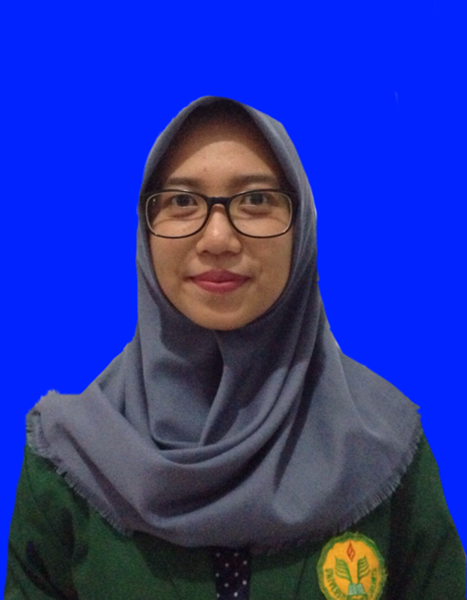
\includegraphics[width=0.27\textwidth]{gambar/pas-foto}
	\end{center}
	\vspace{-80pt}
\end{wrapfigure}

\noindent \textbf{MAULANA RAHMAN NUR.}  Lahir di Jakarta, 17 Juli 1997  Anak pertama dari pasangan Bapak Usep Muhammad Sigih dan Ibu Yuni Puspito Rini. Saat ini beralamatkan di Jl. Olah Raga I RT.010 RW.05 No.64, Cililitan Jakarta Timur.

\vspace{0.5cm}
\noindent
\begin{center}
	\begin{flushright}
		\begin{tabular}{lcl}
			No. Ponsel	& :&  081280100253 \\
			Email	& :&  maulanarahmannur67@gmail.com
		\end{tabular}
	\end{flushright}
\end{center}
\vspace{0.5cm}

\noindent \textbf{Riwayat Pendidikan} : Penulis mengawali pendidikan di TK As-Saadah pada tahun 2001 - 2002, dan kemudian melanjutkan pendidikan di SDN Cililitan 01 Pagi pada tahun 2002 - 2008. Setelah itu, penulis melanjutkan ke SMPN 150 Jakarta hingga tahun 2011. Kemudian melanjutkan ke SMAN 14 Jakarta pada tahun 2011-2014. Di Tahun 2014 penulis melanjutkan ke Universitas Negeri Jakarta (UNJ), Program Studi Ilmu Komputer, melalui jalur PENMABA. Di akhir tahun 2018 (Kamis, 09 Agustus 2018) penulis telah memperoleh gelar Sarjana Komputer (S.Kom), Program Studi Ilmu Komputer, Fakultas Matematika dan Ilmu Pengetahuan Alam, Universitas Negeri Jakarta.

\noindent \textbf{Riwayat Organisasi} : Selama di bangku perkuliahan, penulis aktif di organisasi keilmiahan Prograsm Studi Ilmu Komputer sebagai anggota merangkap Sekertaris periode 2015-2016. Penulis juga berpartisipasi dalam kegiatan BINER (Be Innovative and Educated Researcher) yaitu kegiatan workshop dan seminar yang diadakan oleh DEFAULT, dimana penulis tergabung sebagai anggota merangkap Sekertaris. 

\end{document}